\chapter{観測データ解析 \label{chapObs}}

第\ref{chapMock}章では模擬データの解析からいくつかの効果の解析結果への影響を調べた。その結果、asymmetric driftの効果が非常に大きく影響することが分かった。また、他の効果について大きな影響はなく、あまり気にする必要はないと考えらえる。以上の結果を踏まえて、観測データの解析を行う。\ref{観測データ}では、本論文の解析で用いた観測データについて説明する。\ref{使用するサンプル}では観測データの中から実際に解析で使用するサンプルについて説明する。\ref{asymmetric driftを考慮しない場合の解析}、\ref{asymmetric driftを考慮する場合の解析}では、そのように選んできたサンプルを解析した結果を記述する。

\section{観測データ \label{観測データ}}
本研究では\cite{SD18}のカタログを用いて観測データの解析を行っている。このカタログはAPOGEE, Gaia-DSO, GALAH, LAMOST, RAVE, SEGUEの分光サーベイから利用できる分光パラメータとGaia Data Release 2 (DR2)で観測されたデータから約300万天体の年齢推定値を含むカタログとなっている。図\ref{fig2}は\cite{SD18}で年齢推定をした星の銀河座標系での分布である。

\cite{SD18}は分光データおよび測光データに等時曲線フィットをすることで年齢推定を行っており、年齢の不定性はAPOGEEで$\sim 16\,\%$(最も正確な分光年齢推定)、GALAHで$\sim 21\,\%$、LAMOSTで$\sim 25\,\%$、RAVEとGESで$\sim 40\,\%$となっている。等時曲線とは、恒星進化の理論から与えられる年齢一定の星をヘルツシュプルング・ラッセル図 (HR図) 上でプロットしたときに結んだ線のことである。この等時曲線を、星の分光データと測光データから書けるプロットにフィッティングをすることで年齢推定をする方法が等時曲線フィットである。
% \begin{table}[htb]
% %\scalebox{0.5}
% %\scriptsize
% \footnotesize
% %\small
% \begin{center}
% \scalebox{0.87}[0.9]{
% \begin{tabular}{|l||c|c|c|c|c|} \hline
%     観測 & 天体数 & 波長 & 分解能 & 使用したパラメータ & 測光データ\\ \hline
%     APOGEE & 250万 & $H$バンド 15200 - 16900\AA & 22500 & $T_{\mathrm{eff}},\log g, \mathrm{[M/H]}$ & $J、H、K_s$ (2MASS)\\
%     LAMOST & 310万 & 可視光(3650 - 9000 \AA) & 1800 & $T_{\mathrm{eff}},\log g, \mathrm{[Fe/H]}$ & $J、H、K_s$ (2MASS) \\
%     RAVE & 50万 & 8400 - 8800 \AA & 7500 & -  & $J、H、K_s$ (2MASS)\\
%     GES & - & - & 20000, 50000 & $T_{\mathrm{eff}},\log g, \mathrm{[Fe/H]}$ & $J_v,H_v,K_v$ (VISTA)、 $J、H、K_s$ (2MASS)\\
%     GALAH & 26万 & - & 28000 & $T_{\mathrm{eff}},\log g, \mathrm{[Fe/H]}$ & $J、H、K_s$ (2MASS)\\
%     SEGUE & 19万 & 可視光 & 2000 & $T_{\mathrm{eff}},\log g, \mathrm{[Fe/H]}$ & $J、H、K_s$ (2MASS)\\ \hline
% \end{tabular}
% }
% \caption{\cite{SD18}のカタログで用いられた分光観測の種類、それぞれのデータの天体数、波長、分解能、年齢推定に使用したパラメータと測光データ。}
% \end{center} \label{spec_dataset}
% \end{table}

\begin{figure}[htbp]
\begin{center}
	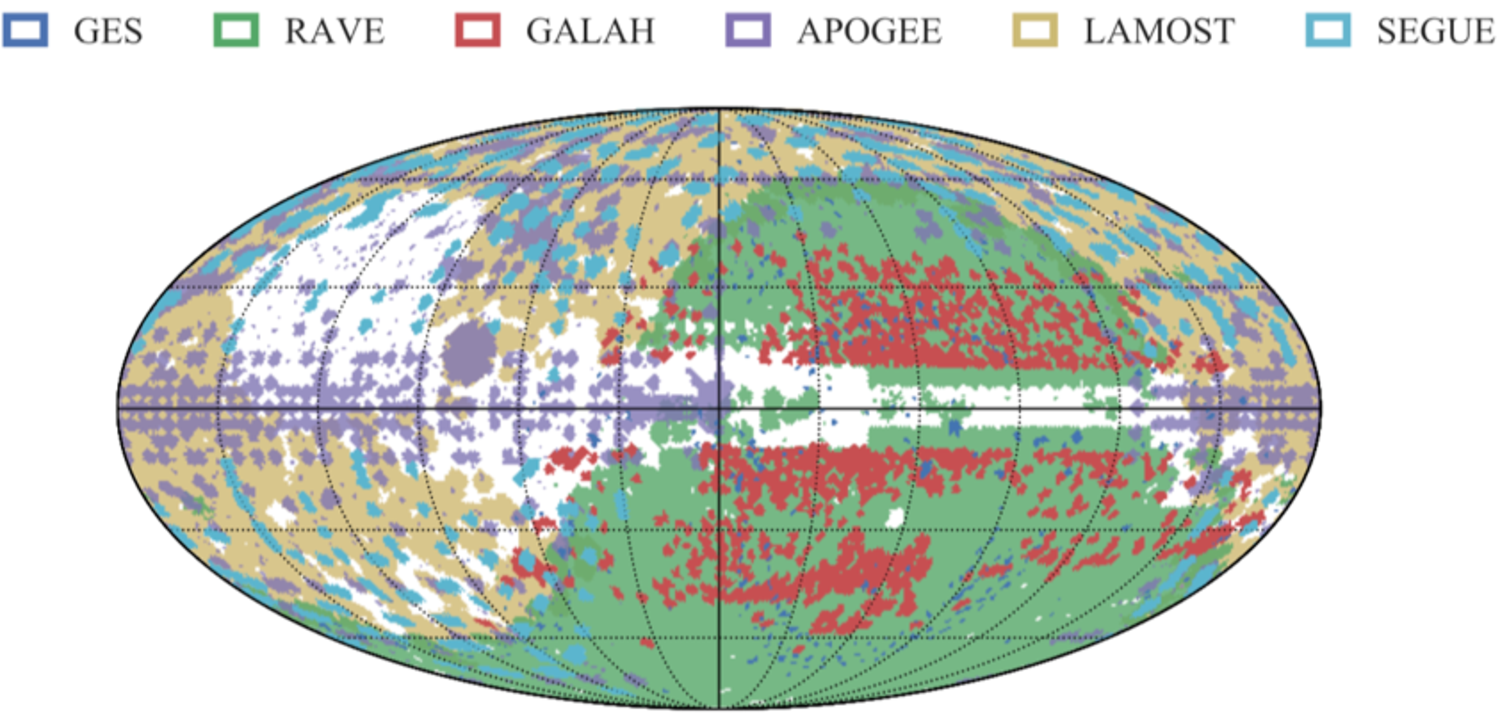
\includegraphics[width=9cm]{fig/SD18_fig1.pdf}
	\caption{\cite{SD18}で年齢推定がなされた星の分布。銀河を見たときのサーベイごとに色付けしている。}
	\label{fig2}
\end{center}
\end{figure}

% 図\ref{mode_plx}、\ref{mode_plx-age}はそれぞれ本研究で使用しているサンプルの年周視差$\varpi$ごとのモードと星の年齢$\tau$ごとのモードである。モードが大きすぎるとモードミキシングを起こしてしまうため、モードが大きくないかどうかを確かめる必要がある。例えば、年周視差$\varpi$がモード1を持っていると太陽運動$U_{\odot}、V_{\odot}、W_{\odot}$に、モード2を持っているとオールト定数$A、B、C、K$に影響してしまう。図\ref{mode_plx}の年周視差ごとのモードでは、$0<\varpi<2\,\si{mas}$では1のモードが-50\%、2のモードが約40\%と大きくなっていることがわかる。$2<\varpi<4\,\si{mas}$、$4<\varpi<6\,\si{mas}$でも1、2のモードの絶対値が約20\%以上と比較的大きい。

% \begin{figure}[htbp]
% \begin{center}
% 	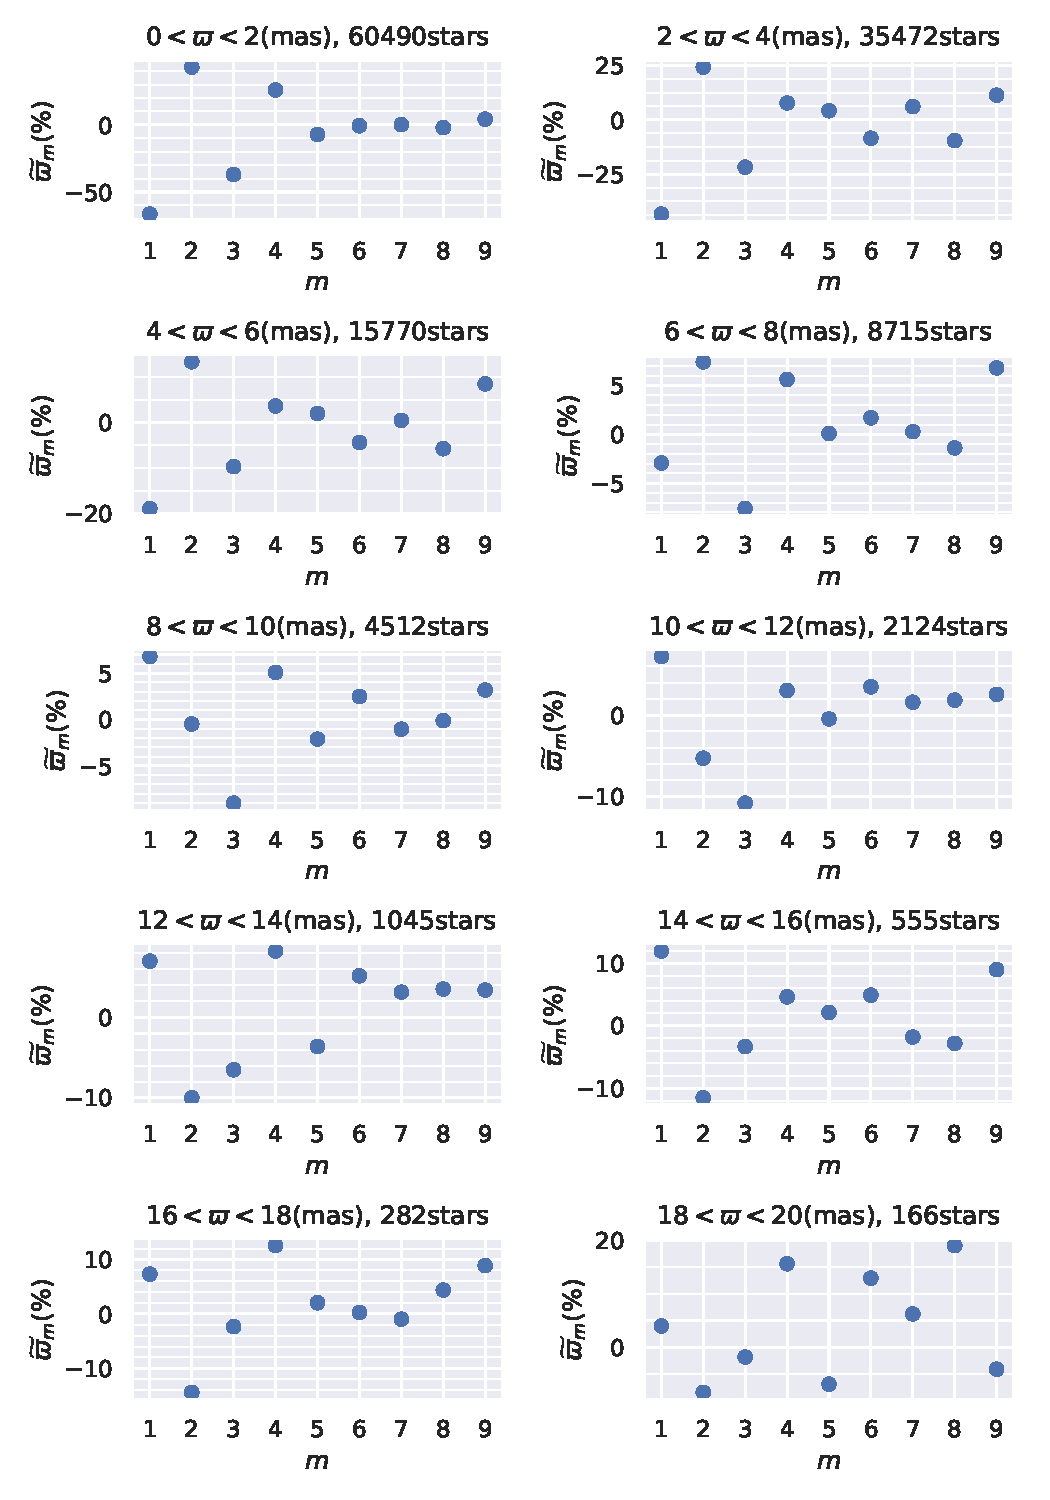
\includegraphics[width=12cm]{fig/mode_plx.pdf}
% 	\caption{今回使用しているサンプルの年周視差2 masごとのモード。各年周視差ごとのサンプルをフーリエ変換している。mはモードの係数である。}
% 	\label{mode_plx}
% \end{center}
% \end{figure}

% \begin{figure}[htbp]
% \begin{center}
% 	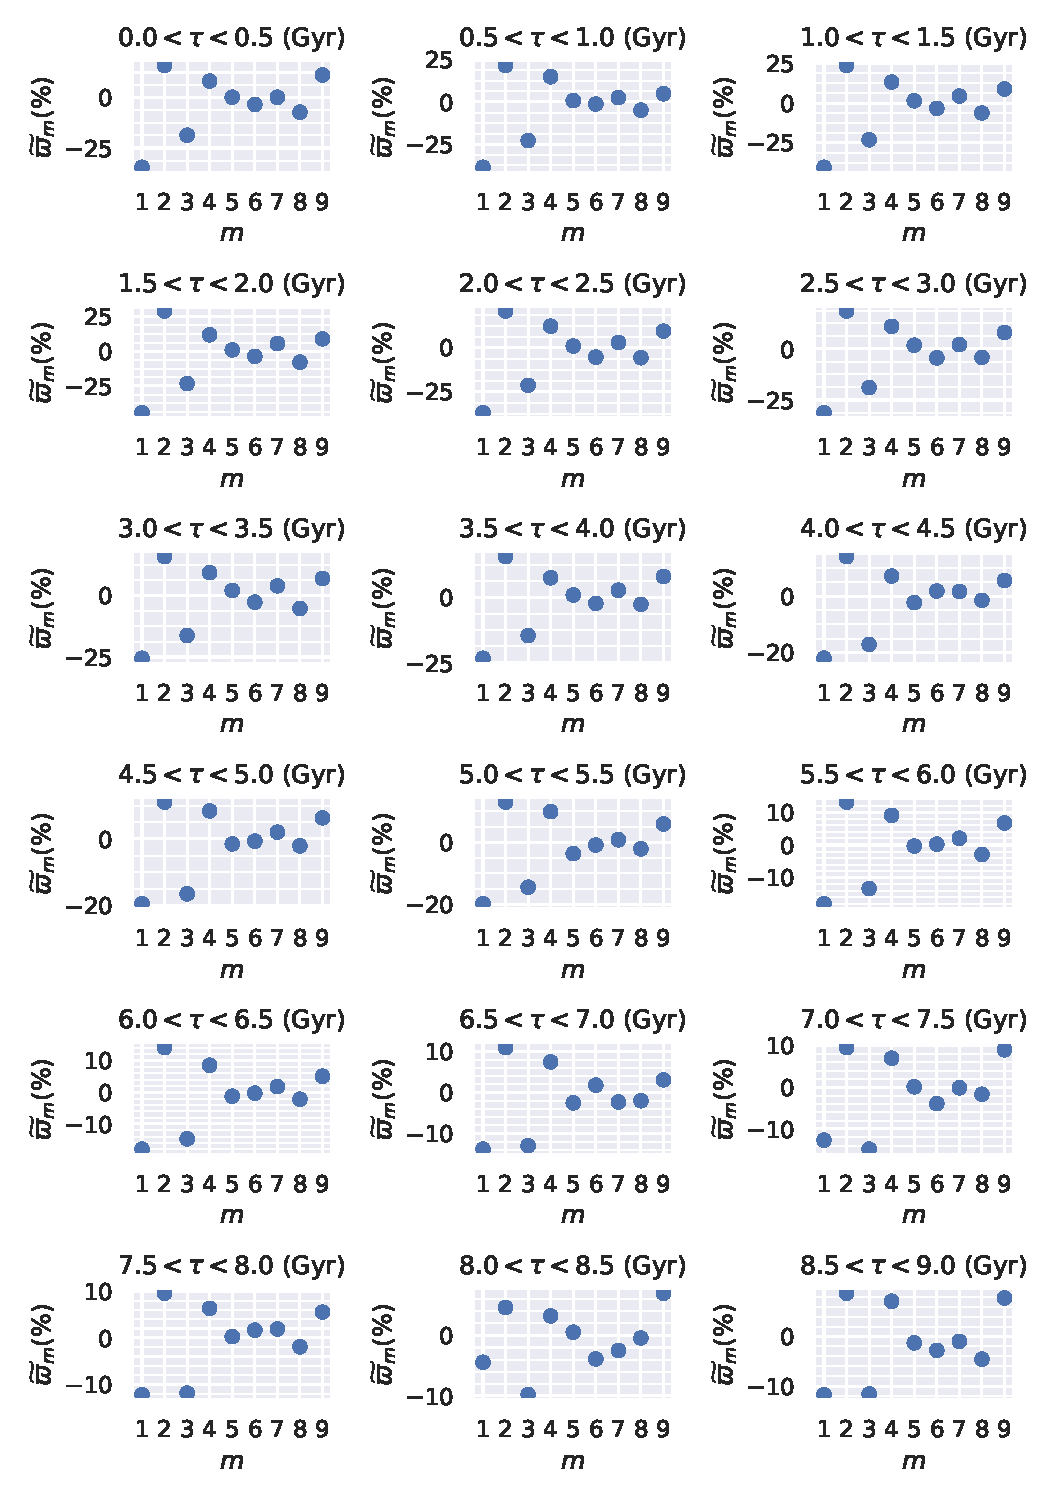
\includegraphics[width=14cm]{fig/mode_plx-age.pdf}
% 	\caption{太陽から1 kpc以内、年周視差の精度20\%以上、速度の観測誤差$3\,\mathrm{km\,s^{-1}}$以下の星の年齢0 Gyrから9 Gyrまでの0.5 Gyrごとのサンプルの年齢ごとのモード。mはモードの係数である。}
% 	\label{mode_plx-age}
% \end{center}
% \end{figure}



% 図\ref{hist_seaborn_50Myr}, \ref{hist_seaborn_200Myr}, \ref{hist_seaborn_1Gyr}は星の年齢ごとの$U,V$の2次元速度分布である。$|z|<100\ \mathrm{pc}$のサンプルを使用している。

% \begin{figure}[htbp]
% \begin{center}
% 	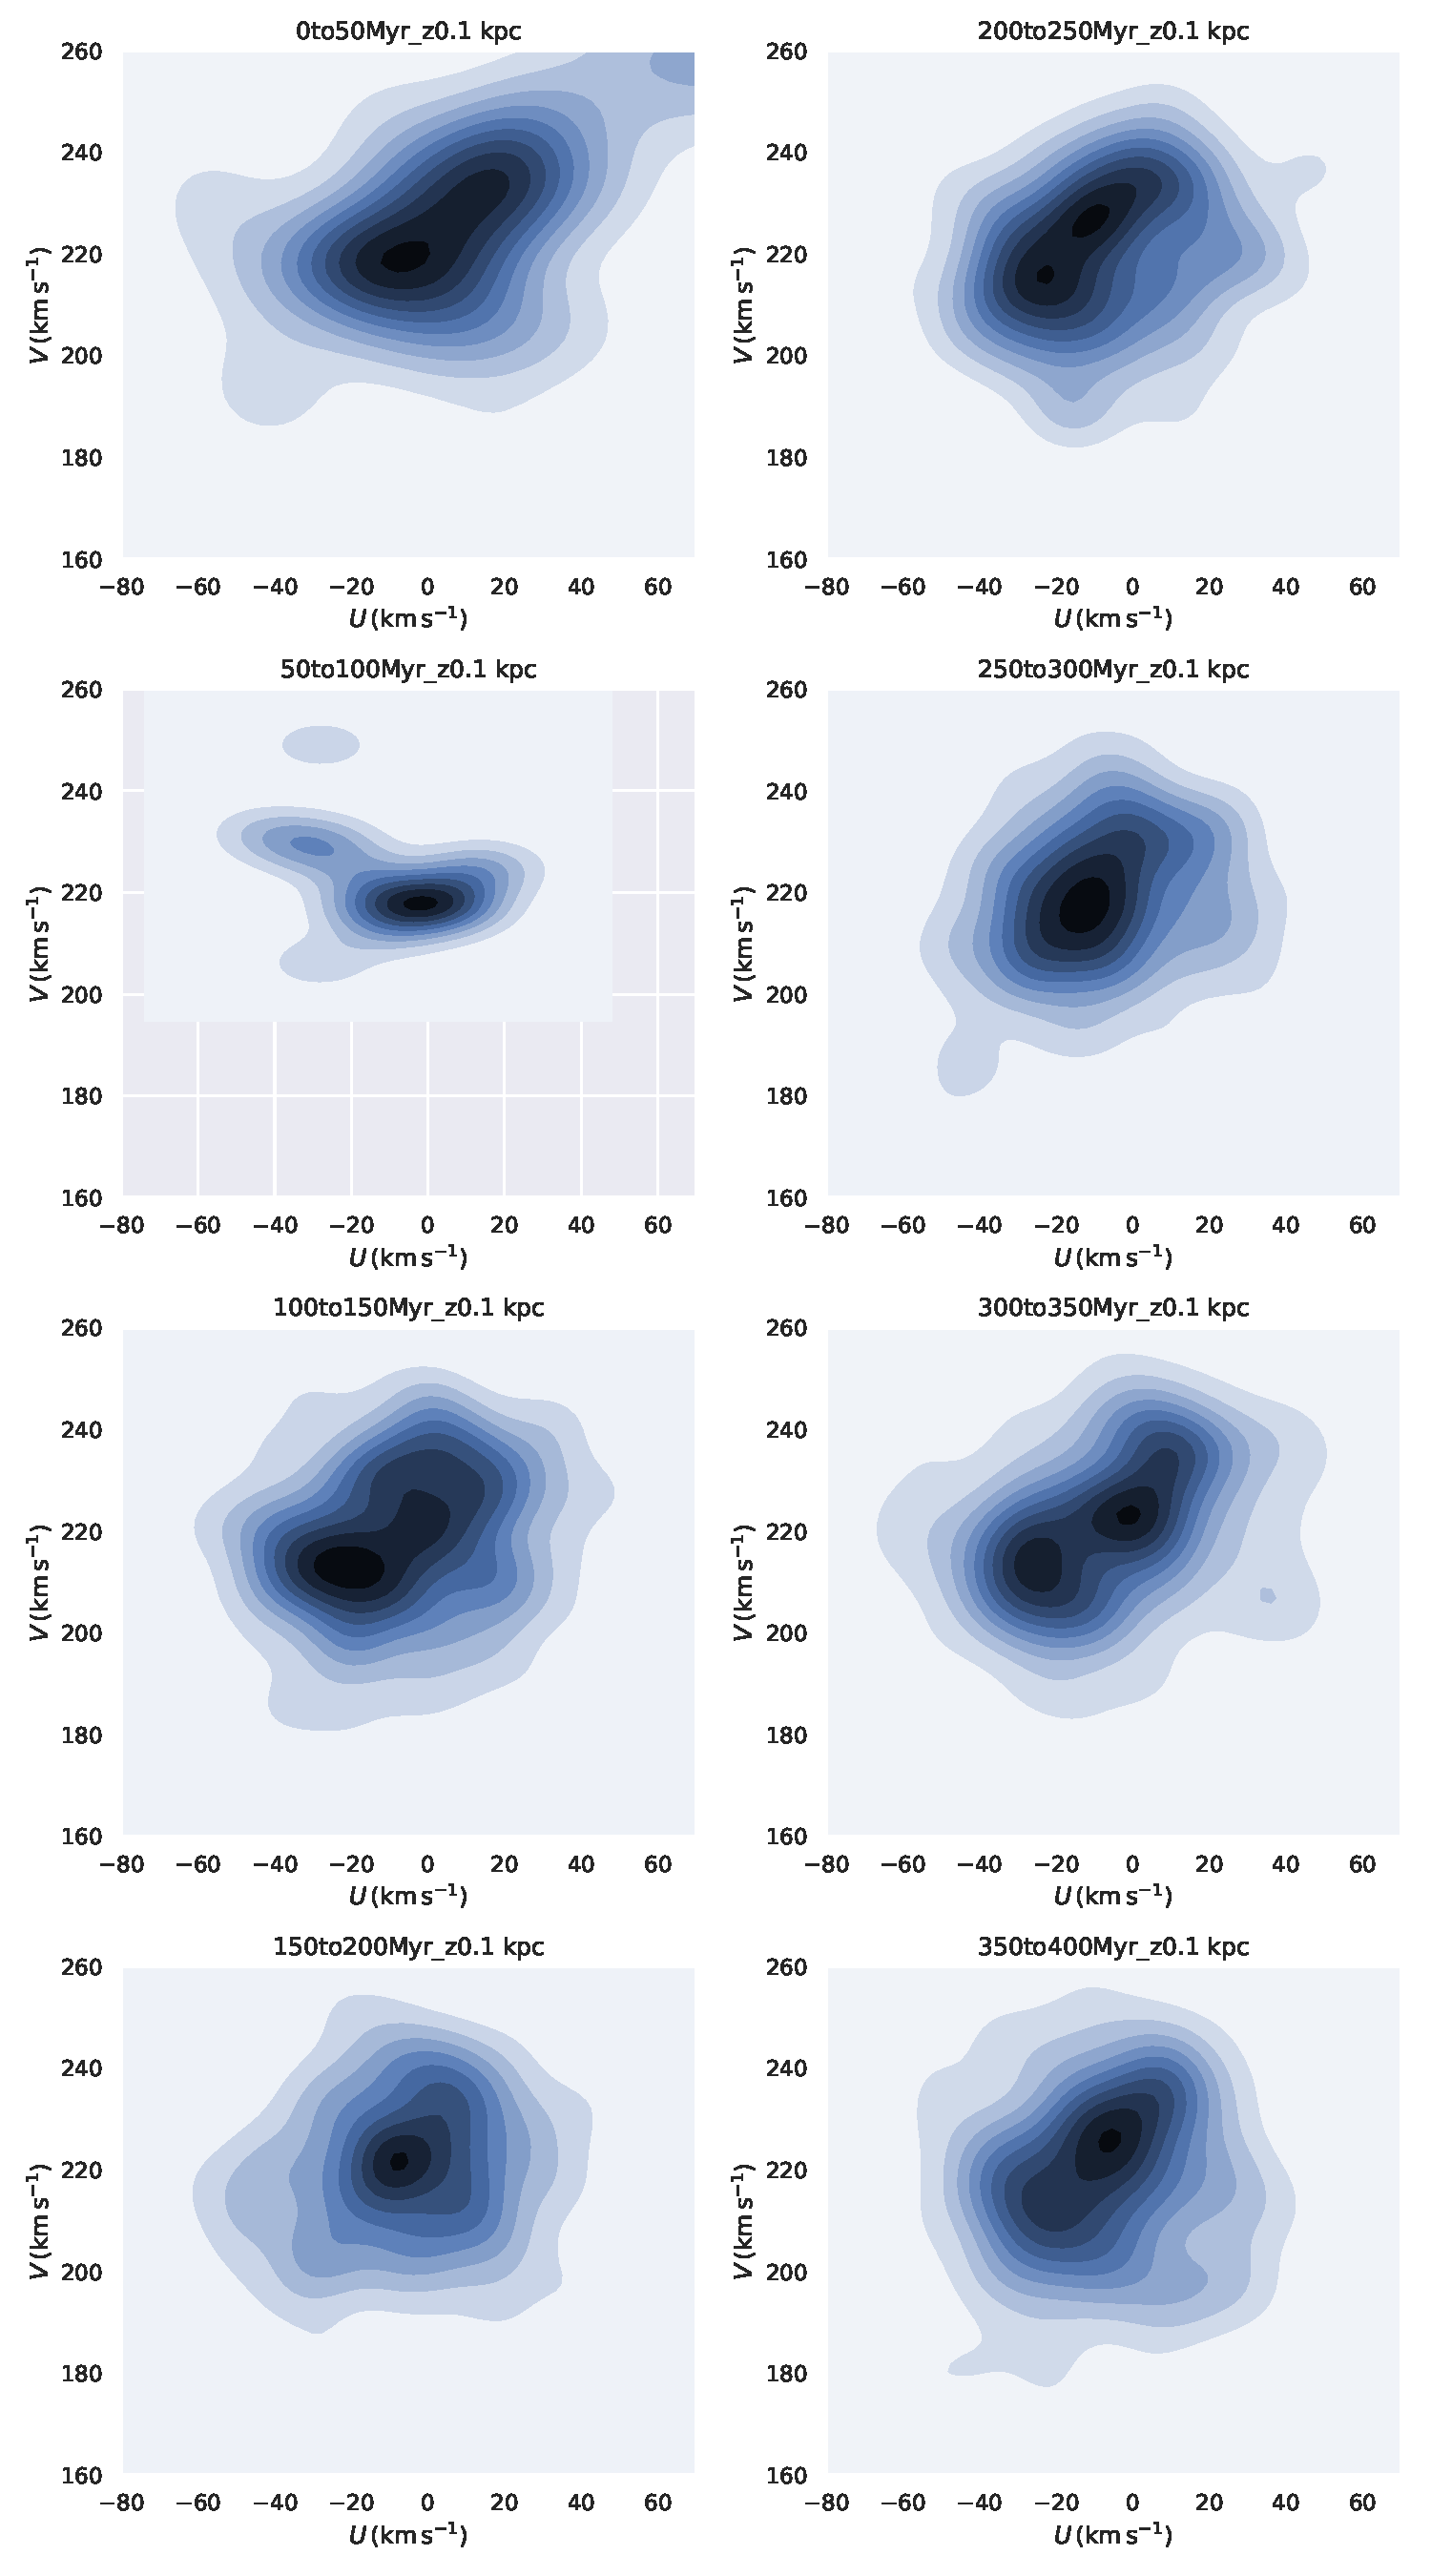
\includegraphics[width=12cm]{fig/UV/hist_seaborn_2_z0.1kpc.pdf}
% 	\caption{太陽から1 kpc以内、年周視差の精度20\%以上、速度の観測誤差$3\,\mathrm{km\,s^{-1}}$以下の星の年齢50 Myrごとの動径方向速度$U$、方位角方向速度$V$の分布。}
% 	\label{hist_seaborn_50Myr}
% \end{center}
% \end{figure}

% \begin{figure}[htbp]
% \begin{center}
% 	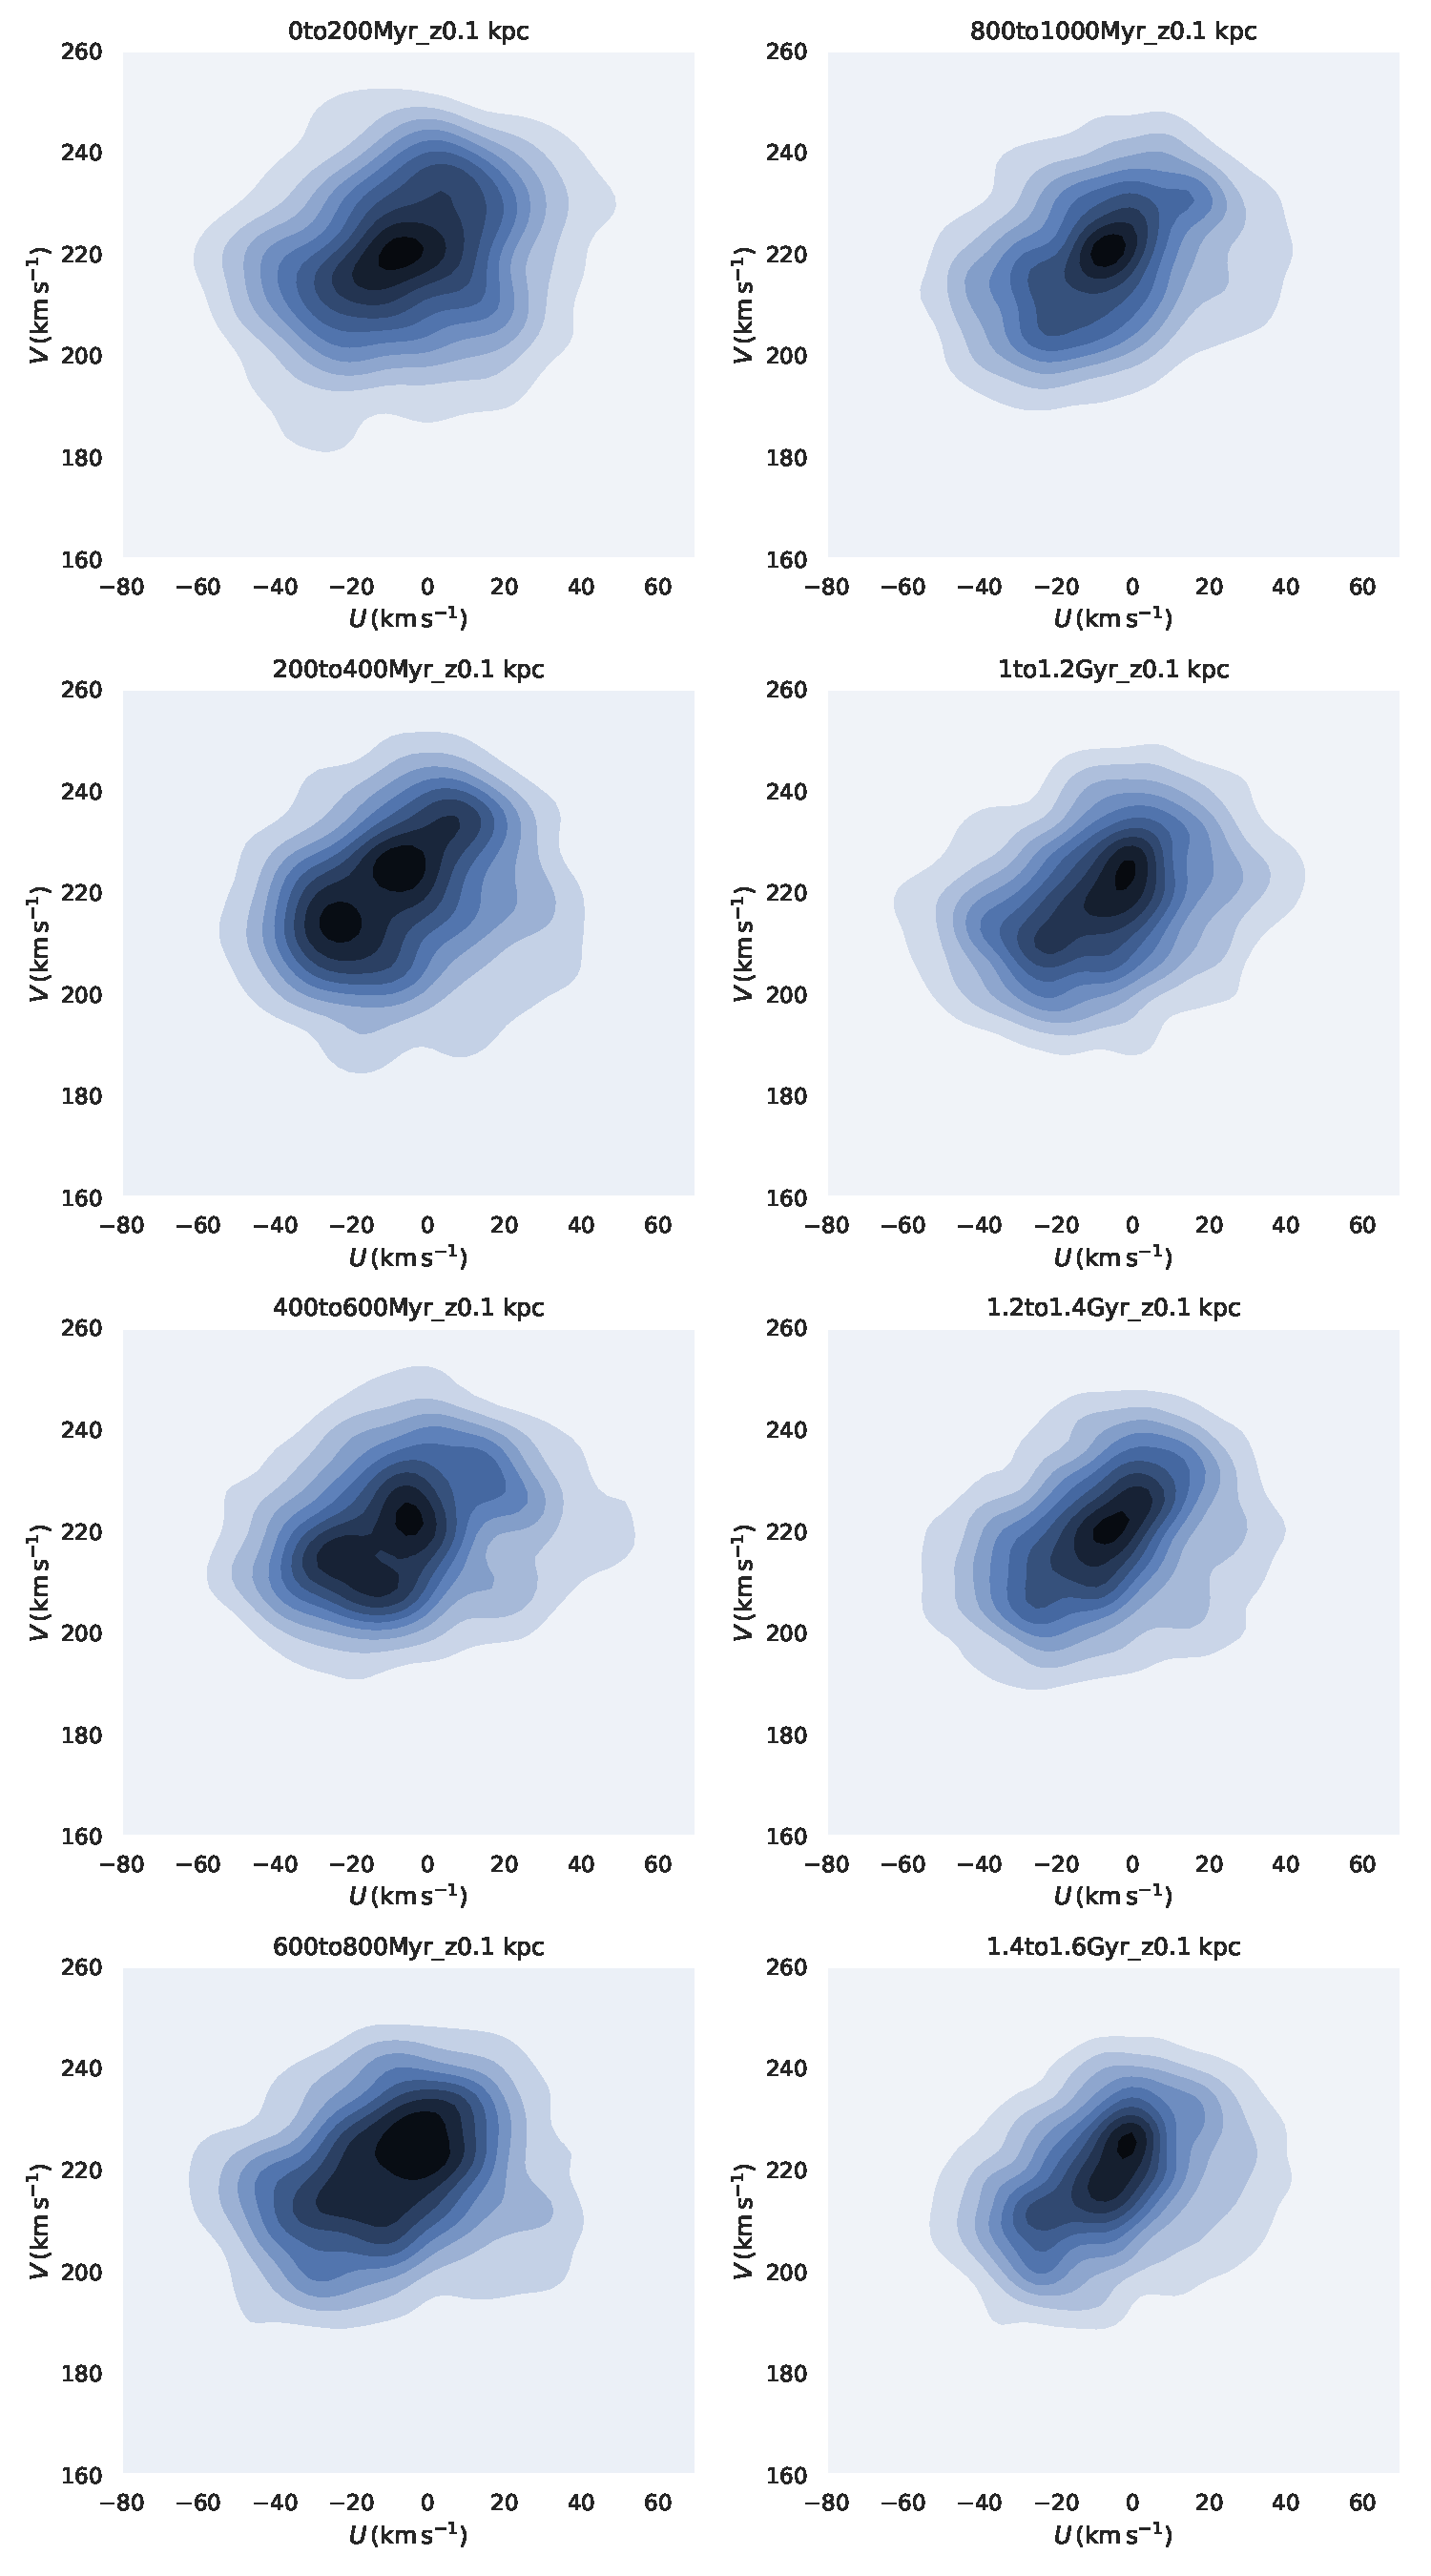
\includegraphics[width=12cm]{fig/UV/hist_seaborn_1_z0.1kpc.pdf}
% 	\caption{太陽から1 kpc以内、年周視差の精度20\%以上、速度の観測誤差$3\,\mathrm{km\,s^{-1}}$以下の星の年齢200 Myrごとの動径方向速度$U$、方位角方向速度$V$の分布。}
% 	\label{hist_seaborn_200Myr}
% \end{center}
% \end{figure}

% \begin{figure}[htbp]
% \begin{center}
% 	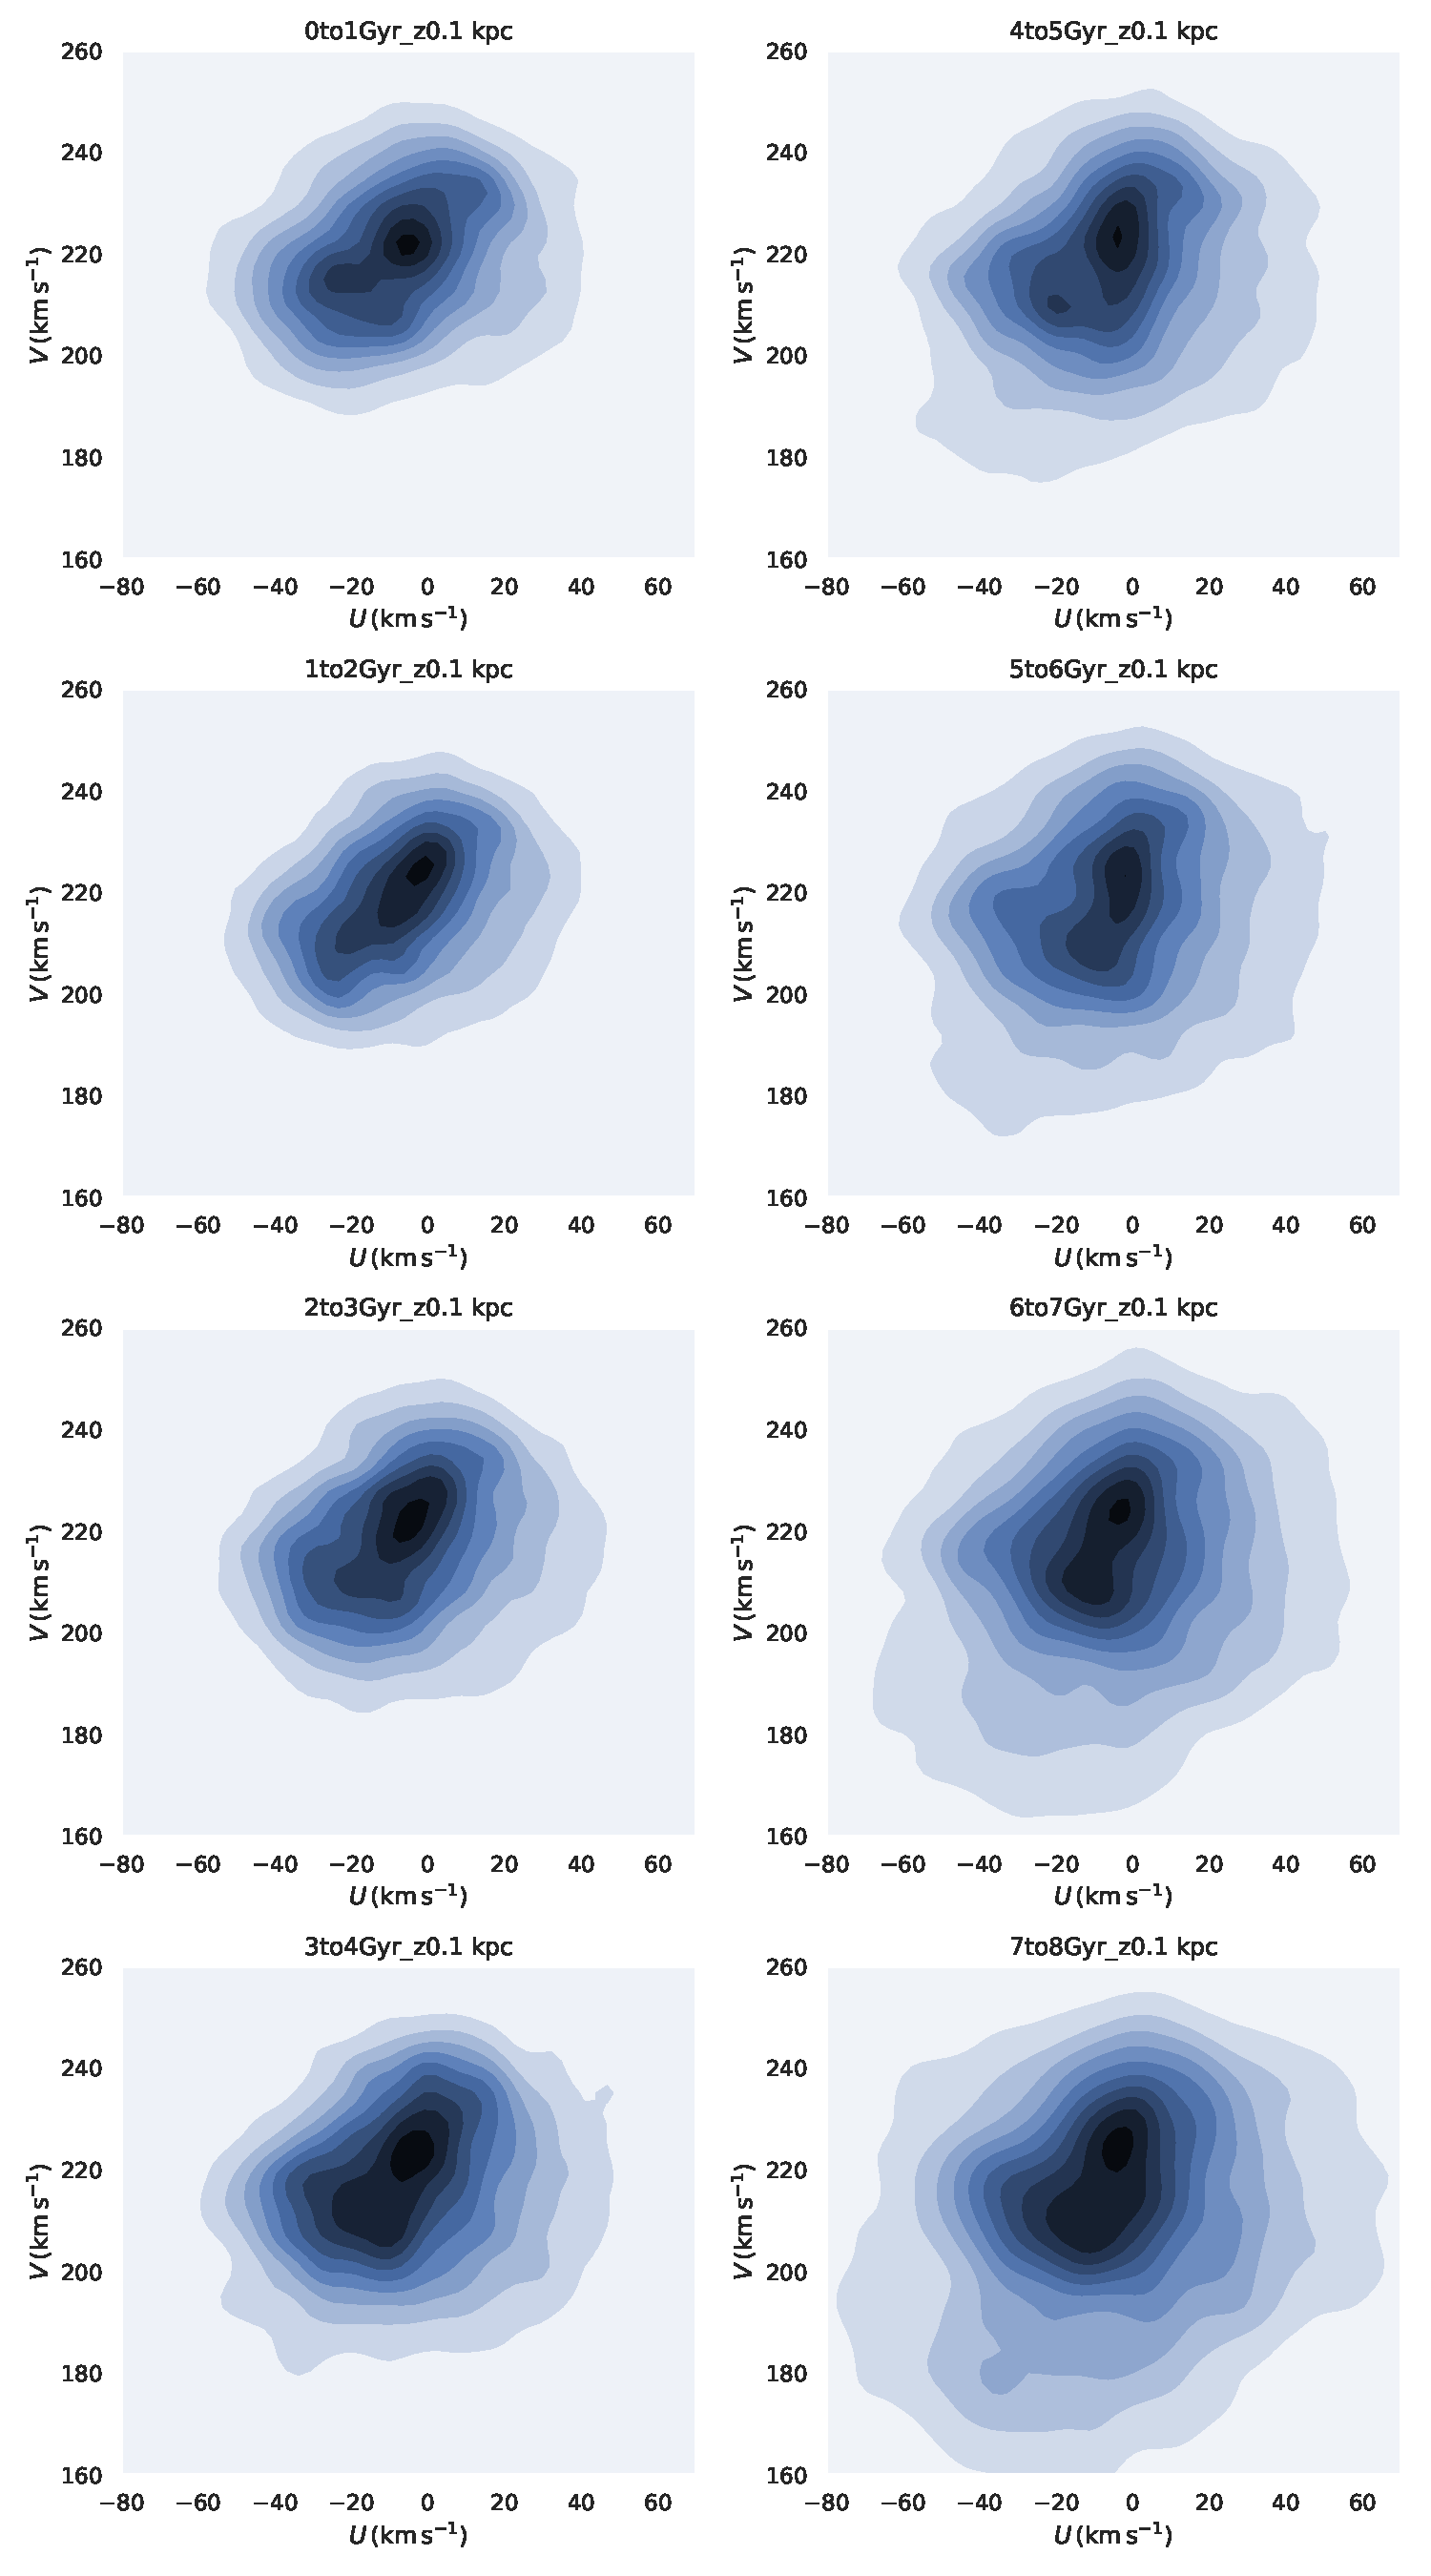
\includegraphics[width=12cm]{fig/UV/hist_seaborn_0_z0.1kpc.pdf}
% 	\caption{太陽から1 kpc以内、年周視差の精度20\%以上、速度の観測誤差$3\,\mathrm{km\,s^{-1}}$以下の星の年齢1 Gyrごとの動径方向速度$U$、方位角方向速度$V$の分布。}
% 	\label{hist_seaborn_1Gyr}
% \end{center}
% \end{figure}

% 図\ref{hist_UV_50Myr}, \ref{hist_UV_200Myr}, \ref{hist_UV_1Gyr}は図\ref{hist_seaborn_50Myr}, \ref{hist_seaborn_200Myr}, \ref{hist_seaborn_1Gyr}をプロット方法を変えてプロットした図である。

% \begin{figure}[htbp]
%   \centering
% \begin{tabular}{cc}
% 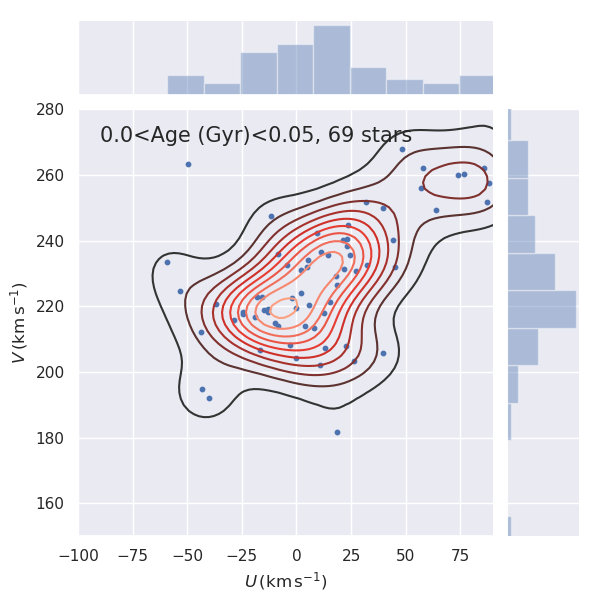
\includegraphics[width=5cm]{fig/UV/0to50Myr_z0.1kpc_hist2d.png}&
% 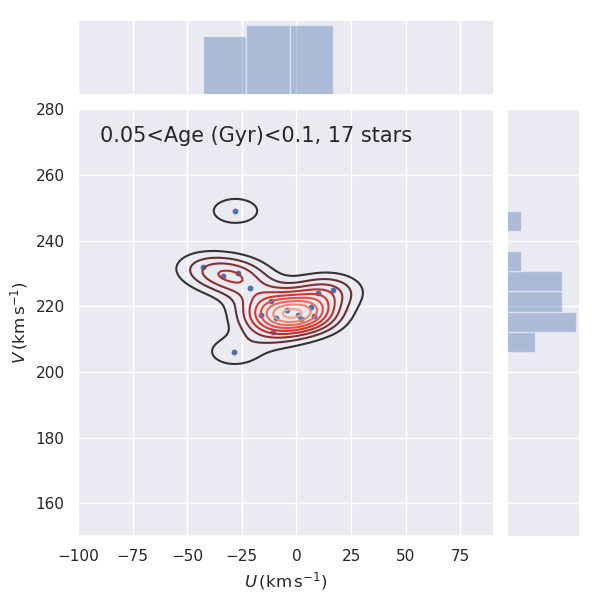
\includegraphics[width=5cm]{fig/UV/50to100Myr_z0.1kpc_hist2d.png}\\
% 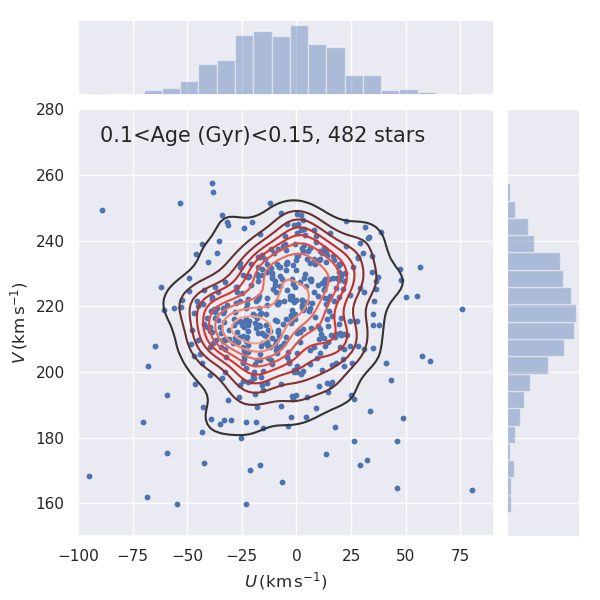
\includegraphics[width=5cm]{fig/UV/100to150Myr_z0.1kpc_hist2d.png}&
% 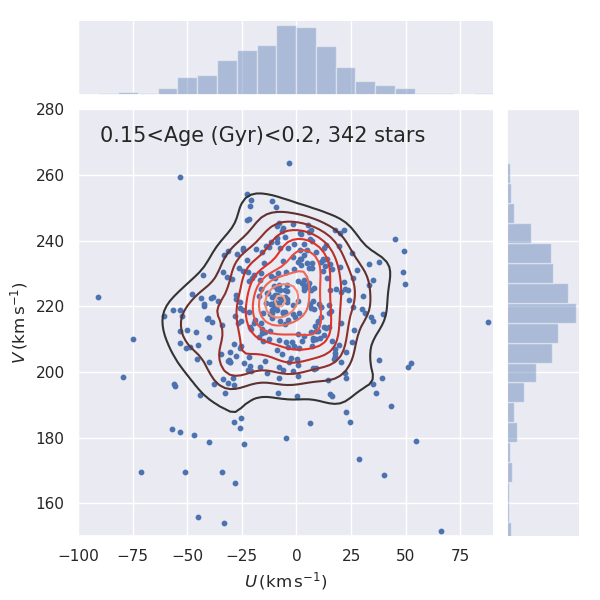
\includegraphics[width=5cm]{fig/UV/150to200Myr_z0.1kpc_hist2d.png}\\
% 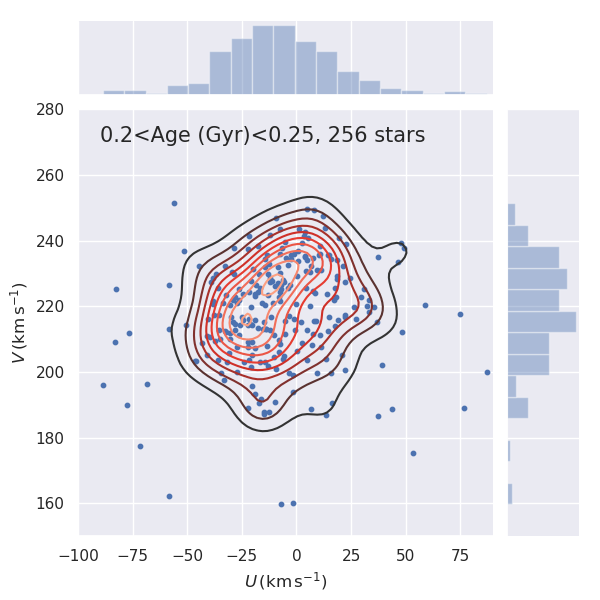
\includegraphics[width=5cm]{fig/UV/200to250Myr_z0.1kpc_hist2d.png}&
% 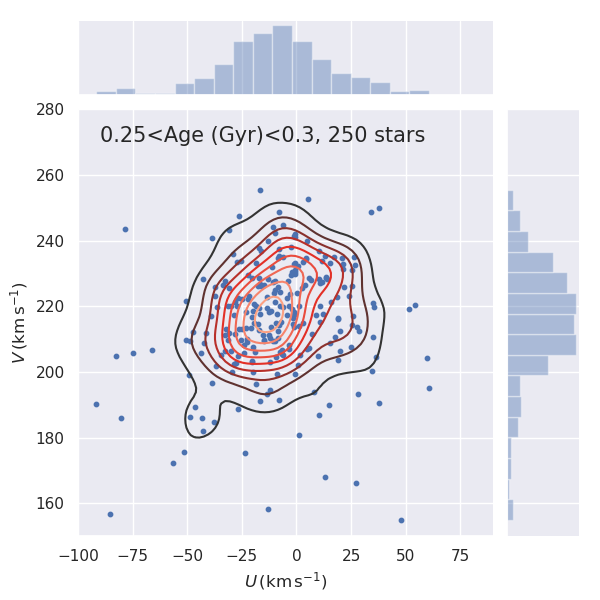
\includegraphics[width=5cm]{fig/UV/250to300Myr_z0.1kpc_hist2d.png}\\
% 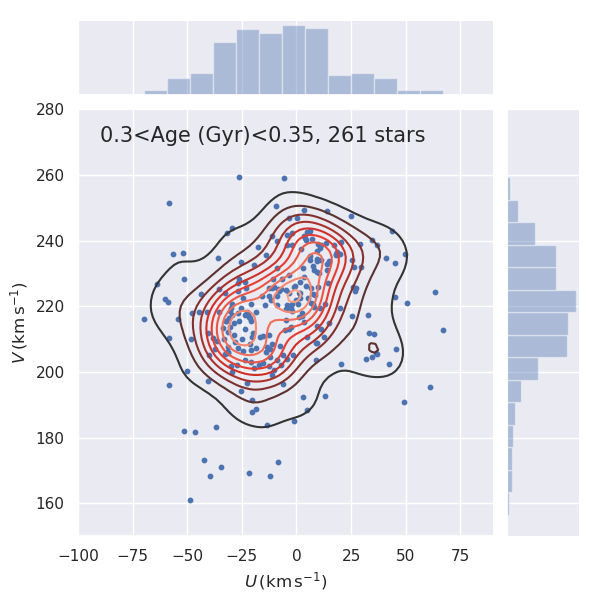
\includegraphics[width=5cm]{fig/UV/300to350Myr_z0.1kpc_hist2d.png}&
% 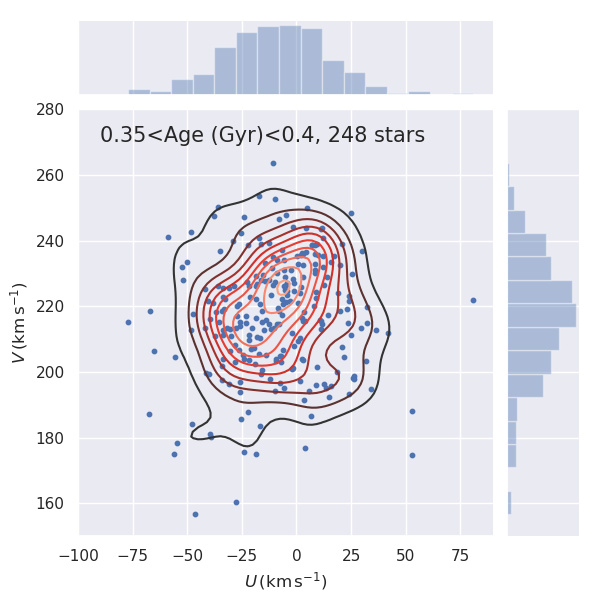
\includegraphics[width=5cm]{fig/UV/350to400Myr_z0.1kpc_hist2d.png}\\
% \end{tabular}
%     \caption{太陽から1 kpc以内、年周視差の精度20\%以上、速度の観測誤差$3\,\mathrm{km\,s^{-1}}$以下の星の年齢50 Myrごとの動径方向速度$U$、方位角方向速度$V$の分布。}
%     \label{hist_UV_50Myr}
% \end{figure}

% \begin{figure}[htbp]
%   \centering
% \begin{tabular}{cc}
% 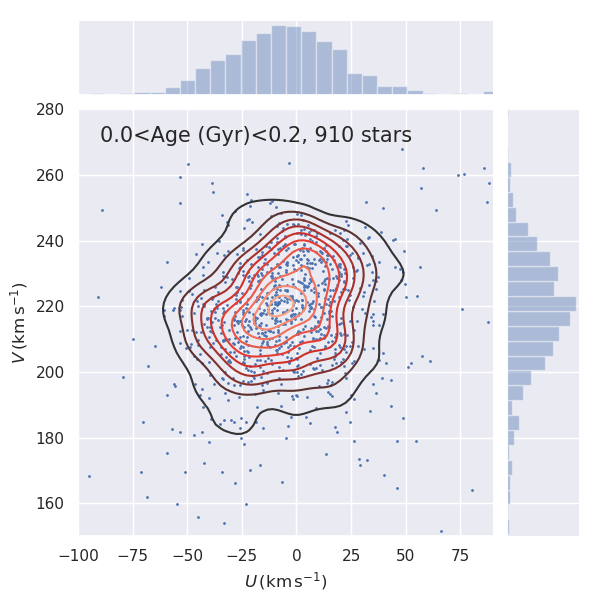
\includegraphics[width=5cm]{fig/UV/0to200Myr_z0.1kpc_hist2d.png}&
% 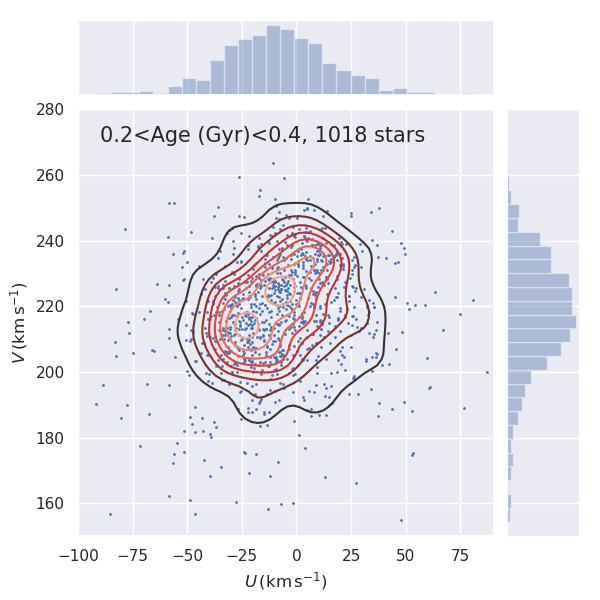
\includegraphics[width=5cm]{fig/UV/200to400Myr_z0.1kpc_hist2d.png}\\
% 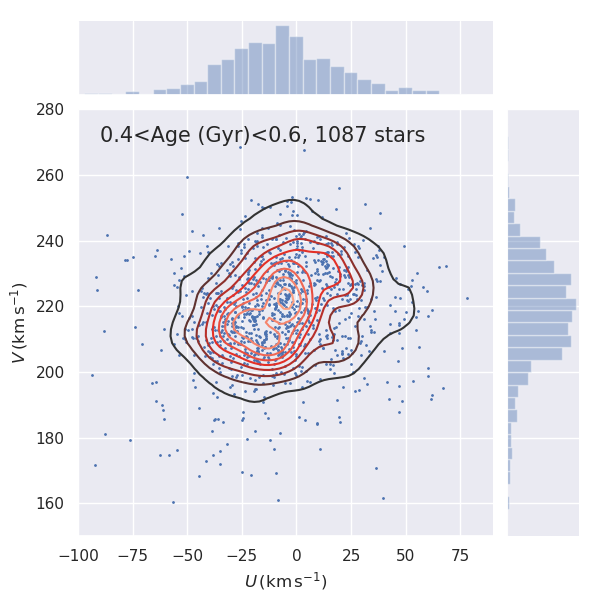
\includegraphics[width=5cm]{fig/UV/400to600Myr_z0.1kpc_hist2d.png}&
% 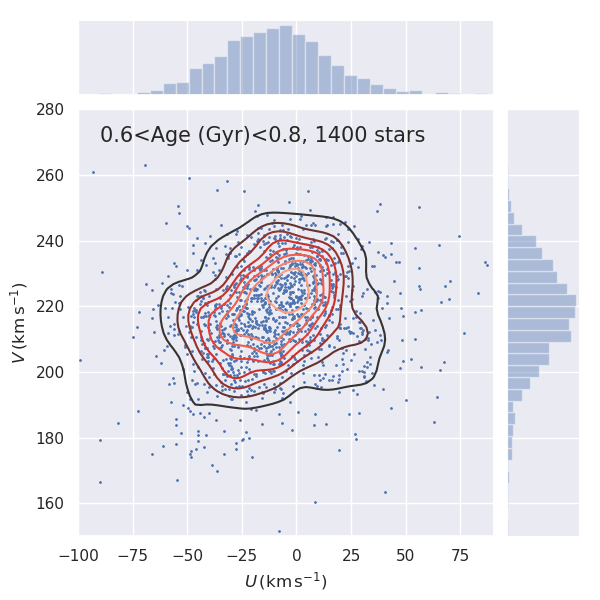
\includegraphics[width=5cm]{fig/UV/600to800Myr_z0.1kpc_hist2d.png}\\
% 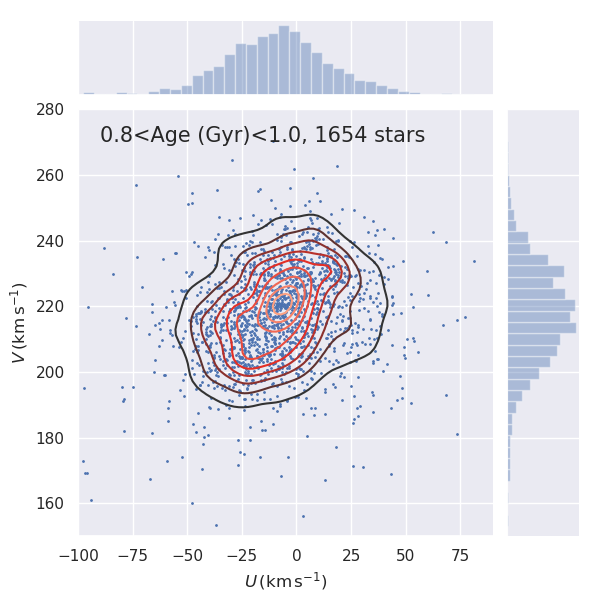
\includegraphics[width=5cm]{fig/UV/800to1000Myr_z0.1kpc_hist2d.png}&
% 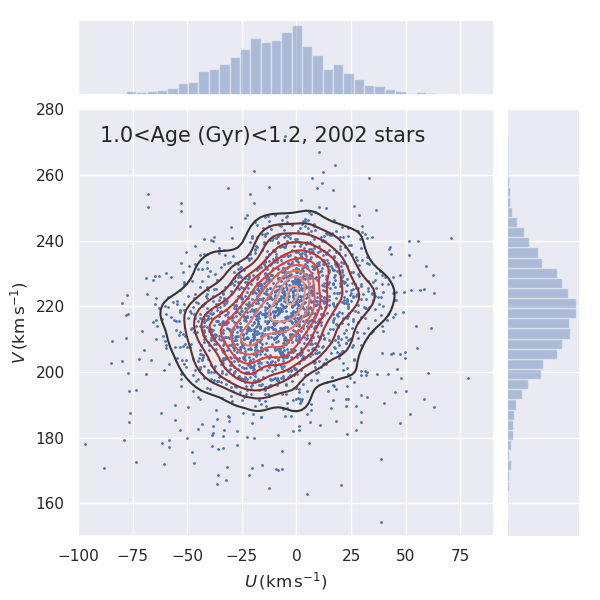
\includegraphics[width=5cm]{fig/UV/1to1.2Gyr_z0.1kpc_hist2d.png}\\
% 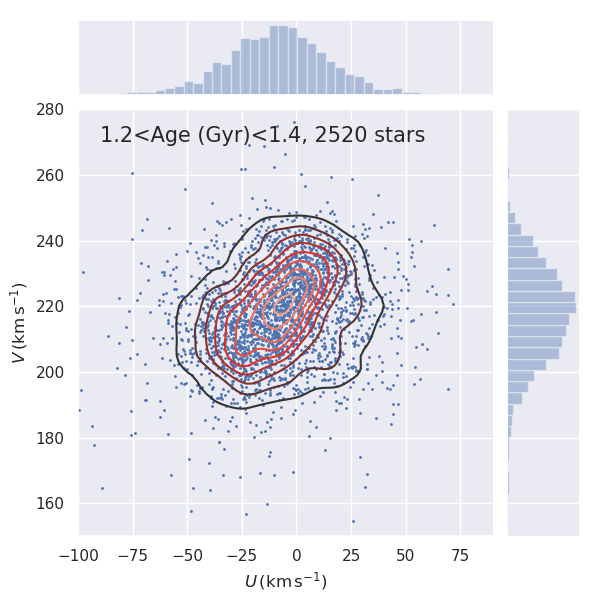
\includegraphics[width=5cm]{fig/UV/1.2to1.4Gyr_z0.1kpc_hist2d.png}&
% 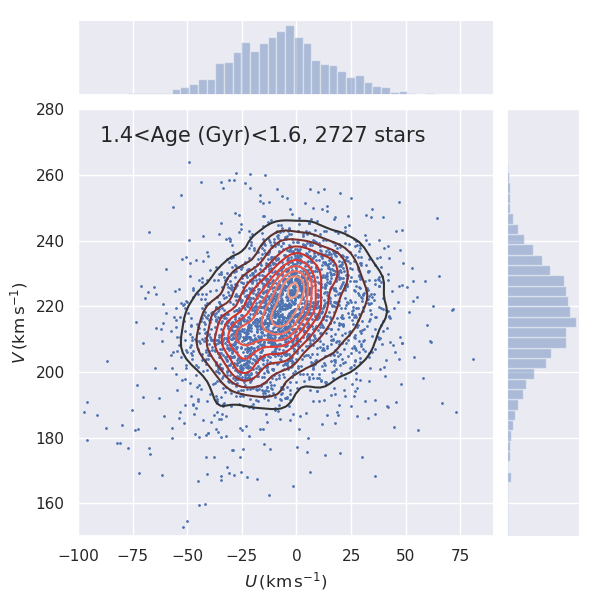
\includegraphics[width=5cm]{fig/UV/1.4to1.6Gyr_z0.1kpc_hist2d.png}\\
% \end{tabular}
%     \caption{太陽から1 kpc以内、年周視差の精度20\%以上、速度の観測誤差$3\,\mathrm{km\,s^{-1}}$以下の星の年齢200 Myrごとの動径方向速度$U$、方位角方向速度$V$の分布。}
%     \label{hist_UV_200Myr}
% \end{figure}

% \begin{figure}[htbp]
%   \centering
% \begin{tabular}{cc}
% 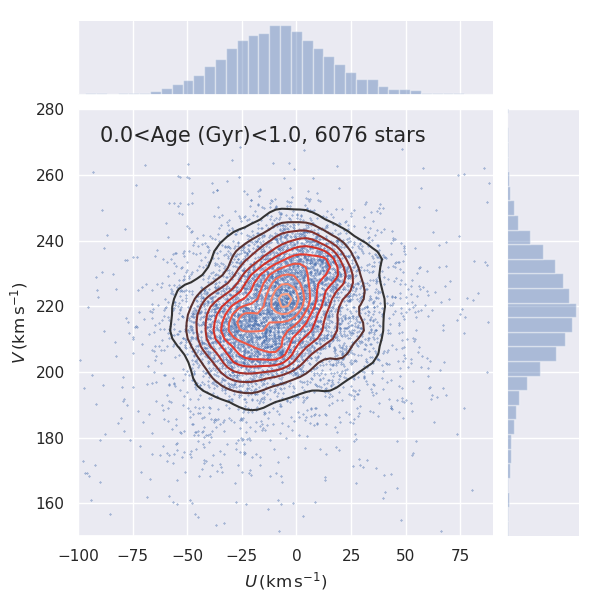
\includegraphics[width=5cm]{fig/UV/0to1Gyr_z0.1kpc_hist2d.png}&
% 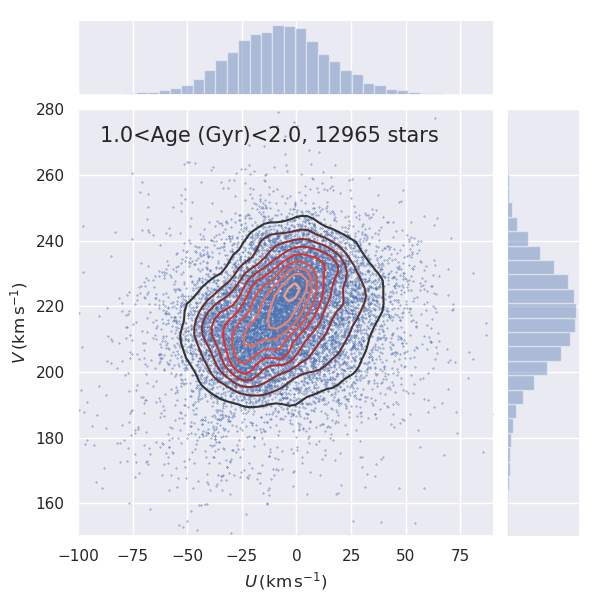
\includegraphics[width=5cm]{fig/UV/1to2Gyr_z0.1kpc_hist2d.png}\\
% 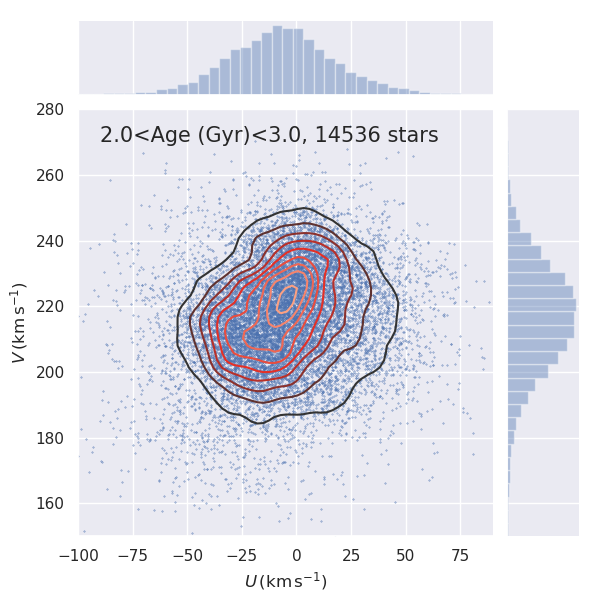
\includegraphics[width=5cm]{fig/UV/2to3Gyr_z0.1kpc_hist2d.png}&
% 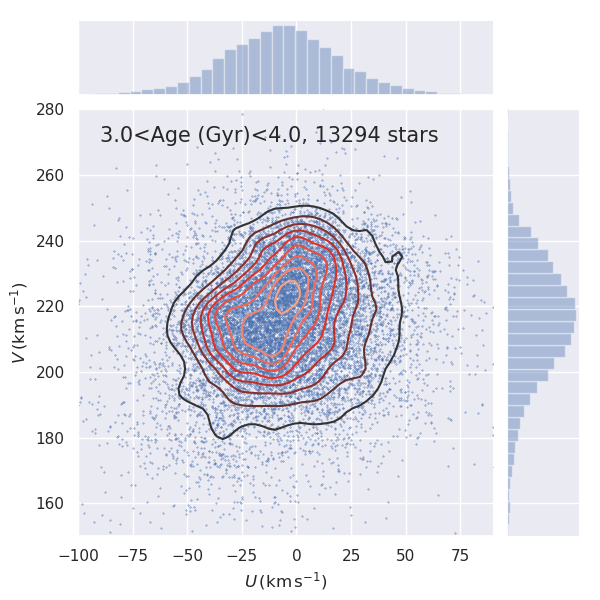
\includegraphics[width=5cm]{fig/UV/3to4Gyr_z0.1kpc_hist2d.png}\\
% 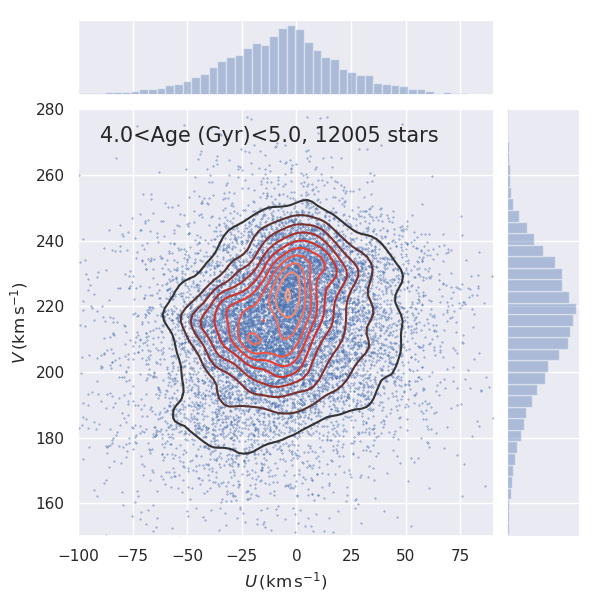
\includegraphics[width=5cm]{fig/UV/4to5Gyr_z0.1kpc_hist2d.png}&
% 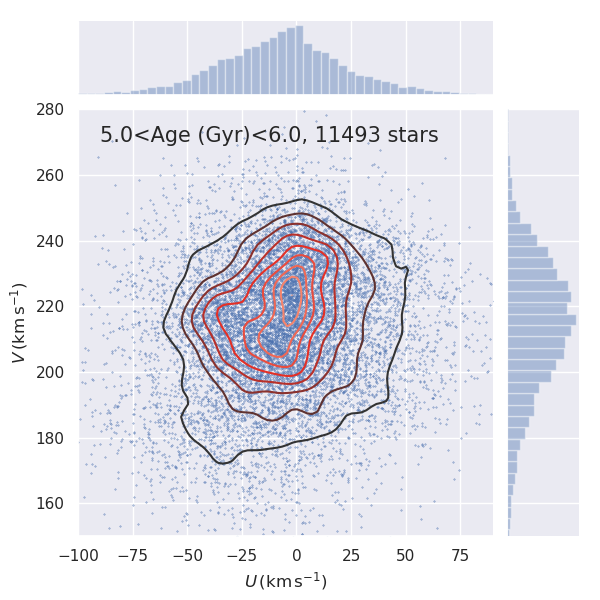
\includegraphics[width=5cm]{fig/UV/5to6Gyr_z0.1kpc_hist2d.png}\\
% 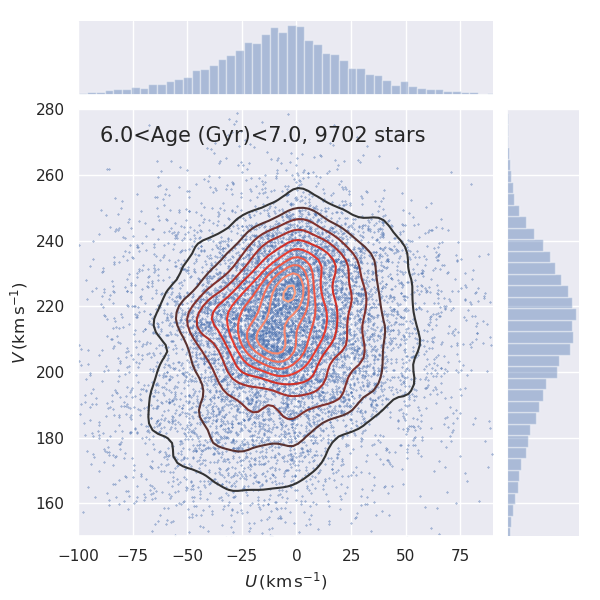
\includegraphics[width=5cm]{fig/UV/6to7Gyr_z0.1kpc_hist2d.png}&
% 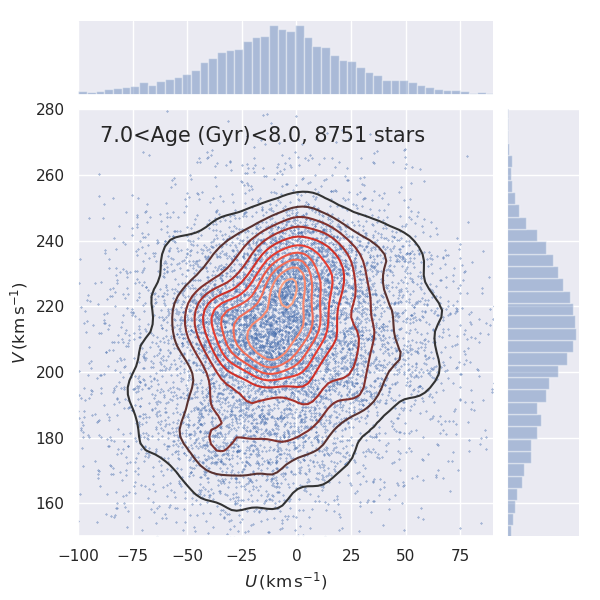
\includegraphics[width=5cm]{fig/UV/7to8Gyr_z0.1kpc_hist2d.png}\\
% \end{tabular}
%     \caption{太陽から1 kpc以内、年周視差の精度20\%以上、速度の観測誤差$3\,\mathrm{km\,s^{-1}}$以下の星の年齢1 Gyrごとの動径方向速度$U$、方位角方向速度$V$の分布。}
%     \label{hist_UV_1Gyr}
% \end{figure}


\subsection{使用するサンプル \label{使用するサンプル}}
年周視差の相対誤差は$\varpi/\sigma_{\varpi}>5$として、20 $\%$未満としている(\cite{BJ15})。速度の観測誤差は、$\mu_l,\mu_b,v_{\mathrm{los}},\varpi$の誤差伝播を考慮して3次元速度ベクトル$v_{\mathrm{Total}}$と誤差を計算して$\sigma_{v_{\mathrm{Total}}}<3\,\mathrm{km\,s^{-1}}$と制限している。本研究で用いているOort-Lindbladモデルは冷たい系を考えているため、薄い円盤星(thin disk star)に適用したい。薄い円盤は典型的に金属量[Fe/H]$>-0.4\,\mathrm{dex}$、年齢$\tau<\SI{10}{Gyr}$、円盤面からの距離300\,pc以内の星の星であることから、本論文では[Fe/H]$>-0.2\,\mathrm{dex}$、円盤面からの距離$|z|<100\,\mathrm{pc}$、星の年齢$\tau < 8\,\mathrm{Gyr}$のサンプルを用いている。表\ref{dataset}は本論文で用いた観測データのサンプル数である。図\ref{fig:v_sigma}はサンプルの平均速度と速度分散のプロットである。この図を見ると、$\overline{V_{\phi}}$は太陽から遠い星を計算に含めるほど小さくなり、また星の年齢が上がるにつれて低くなっている。また、若い星のサンプルでは太陽からと遠い範囲のサンプルの方が$\overline{V_R}$の値が大きい。$\overline{V_z}$は太陽からの距離が近いサンプルの方が大きい値になっている。速度分散に関してはサンプル間で大きな差はないが、強い年齢依存性が見られる。また、0 - 1 Gyrでは2 Gyrより古い星と比べて平均速度と速度分散の各成分で異なる傾向が見られる。

また、この観測データ解析では太陽から銀河中心までの距離は$R_{\odot} = 8.2\pm 0.1\ \mathrm{kpc}$(\cite{BH2016})としている。また、VLBIの観測(\cite{RB04},\cite{Reid08})からいて座A$^*$に対する太陽の接線速度は$\Omega_{g,\odot} = 30.24 \pm 0.12\,\mathrm{km\,s^{-1}\,kpc^{-1}}$としている。



\begin{table}
\small
\begin{center}
\scalebox{0.87}[0.9]{
\begin{tabular}{|l|cccccccc|} \hline
    星の年齢 (Gyr) & 0 - 1 & 1 - 2 & 2 - 3 & 3 - 4 & 4 - 5 & 5 - 6 & 6 - 7 & 7 - 8\\ \hline
    $D<400\ \mathrm{pc}$のサンプル数& 3153 & 4746 & 6771 & 7505 & 7314 & 7391 & 6565 & 6108\\
    $D<700\ \mathrm{pc}$のサンプル数 & 4601 & 9044 & 11587 & 11354 & 10631 & 10480 & 8939 & 8152\\
    $D<1\ \mathrm{kpc}$のサンプル数  & 6076 & 12965 & 14537 & 13296 & 12036 & 11554 & 9768 & 8821\\ \hline
\end{tabular}
}
\caption{使用したサンプルの星の年齢と太陽からの距離の範囲でのそれぞれのサンプル数}
\label{dataset}
\end{center}
\end{table}


\begin{figure}[p]
\begin{center}
	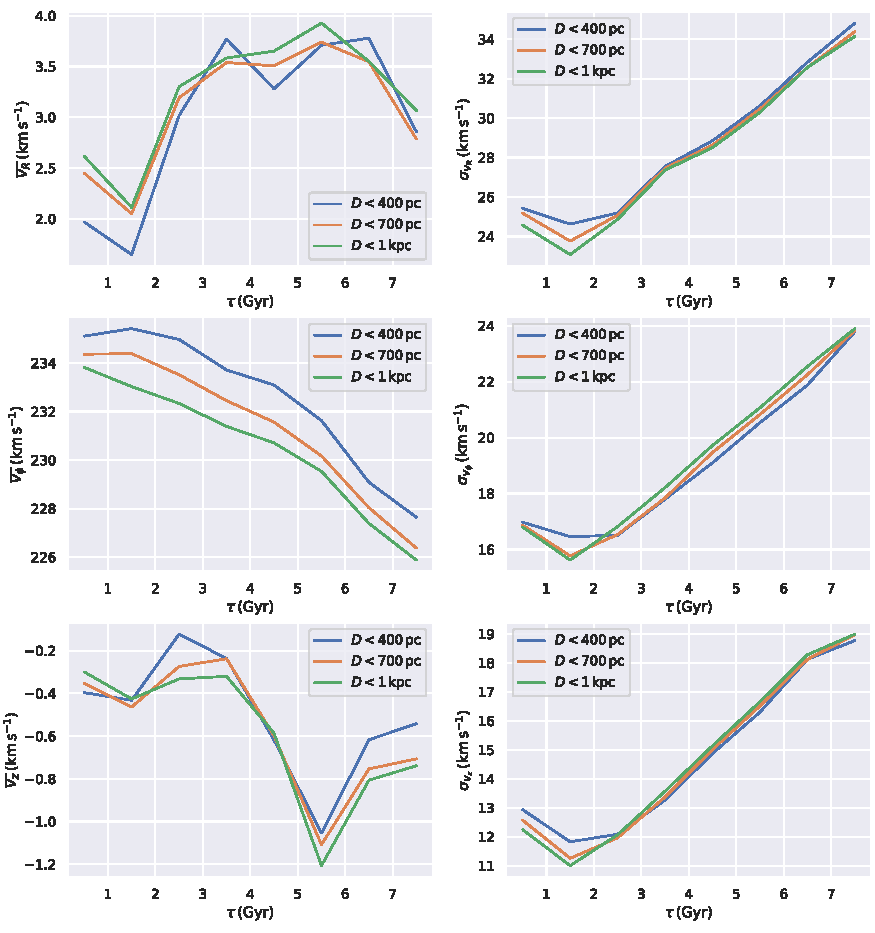
\includegraphics[width=15cm]{fig/v_sigma.pdf}
	\caption{\cite{SD18}のカタログの銀河中心を原点とするときの円筒座標系での平均速度と速度分散。太陽からの距離$\SI{400}{pc}$以内、$\SI{700}{pc}$以内、$\SI{1}{kpc}$以内の3つの範囲の星で計算した。速度の誤差などの他の条件は\ref{使用するサンプル}と同じである。太陽の特異速度は$(U_{\odot},V_{\odot},W_{\odot}) = (11.10,12.24,7.25)\,\si{km.s^{-1}}$ (\cite{Schonrich2010})、LSRの速度は$238\,\si{km.s^{-1}}$ (\cite{BH2016})として星の速度を座標変換している。サンプルの星の年齢を0 - 1 Gyr, 1 - 2 Gyrのように8 Gyrまでで区切っている。左側の列は各年齢での平均速度、右側の列は各年齢での速度分散の値。それぞれの線は使用したサンプルの太陽からの距離の範囲の違いである。}
	\label{fig:v_sigma}
\end{center}
\end{figure}


\section{asymmetric driftを考慮しない場合の解析 \label{asymmetric driftを考慮しない場合の解析}}
第\ref{chapMock}章の模擬データの解析に加えて、本節と次節では以上のように選んだサンプルを解析した結果を示す。本研究では、大きく分けてasymmetirc driftを考慮しない従来の観測方程式(\ref{ObsEq})での解析と考慮した観測方程式(\ref{ObsEqAD})の2種類で観測データ解析を行った。本節では前者のasymmetric driftを考慮しない場合の観測方程式での解析の方法と結果を説明する。

\subsection{解析方法}
まず解析方法について説明する。フィッティングパラメータは$A、\,B、\,C、\,K、\,U_{\odot}、\,V_{\odot}、\,W_{\odot}、\,\sigma_{\mu_l}、\,\sigma_{\mu_b}、\,\sigma_{v_{\mathrm{los}}}$の10個である。$\sigma_{\mu_l}、\,\sigma_{\mu_b}、\,\sigma_{v_{\mathrm{los}}}$はそれぞれ$\mu_l、\,\mu_b、\,v_{\mathrm{los}}$の平均場 (系統速度場)からの速度分散を表す。このとき尤度関数$\mathcal{L}$は
\newpage

\newpage
\begin{align}
\begin{aligned}
	\ln \mathcal{L} =& -\frac{1}{2}\sum_i \left(\frac{\left[\mu_{l,i} - \mu_l^{\mathrm{OL}}(l_i,b_i,\varpi_i)\right]^2}{\sigma_{\mu_l}^2 + (s_{\mu_{l,i}})^2}  + {\rm ln}\left[\sigma_{\mu_l}^2 + (s_{\mu_{l,i}})^2\right] \right. \\
	&+ \frac{\left[\mu_{b,i} - \mu_b^{\mathrm{OL}}(l_i,b_i,\varpi_i)\right]^2}{\sigma_{\mu_b}^2 + (s_{\mu_{b,i}})^2}  + {\rm ln}\left[\sigma_{\mu_b}^2 + (s_{\mu_{b,i}})^2\right] \\
	&+ \frac{\left[v_{\mathrm{los},i} - v^{\mathrm{OL}}_{\mathrm{los}}(l_i,b_i,\varpi_i)\right]^2}{\sigma_{v_{\mathrm{los}}}^2 + (s_{v_{\mathrm{los},i}})^2} + {\rm ln}\left[\sigma_{v_{\mathrm{los}}}^2 + (s_{v_{\mathrm{los},i}})^2\right]\\
	&+ \frac{\left(R_{\odot} - R_{\odot,\mathrm{prior}}\right)^2}{\sigma_{R_{\odot,\mathrm{prior}}}} + \ln{\sigma_{R_{\odot,\mathrm{prior}}}}\\
	&+ \frac{\left(\Omega_{g,\odot} - \Omega_{g,\odot,\mathrm{prior}}\right)^2}{\sigma_{\Omega_{g,\odot,\mathrm{prior}}}} + \ln{\sigma_{\Omega_{g,\odot,\mathrm{prior}}}}\\ 
	&+ \left. \frac{\left(\mu_{b,\mathrm{Sgr\,A}^*} - \mu_{b,\mathrm{Sgr\,A}^*,\mathrm{prior}}\right)^2}{\sigma_{\mu_{b,\mathrm{Sgr\,A}^*,\mathrm{prior}}}} + \ln{\sigma_{\mu_{b,\mathrm{Sgr\,A}^*,\mathrm{prior}}}}\right)
\end{aligned}
\end{align}
と書ける。ここで、添字の$i$は$i$番目の星の値であることを示し、観測量である。また、$s_{\mu_{l,i}},s_{\mu_{b,i}},s_{v_{\mathrm{los},i}}$はそれぞれ$\mu_{l,i},\mu_{b,i},v_{\mathrm{los},i}$の観測誤差である。$\mu_l^{\mathrm{OL}}、\mu_b^{\mathrm{OL}}、v^{\mathrm{OL}}_{\mathrm{los}}$は\ref{観測方程式}の式(\ref{ObsEq})と同じ式を用いている。$R_{\odot}、\Omega_{g,\odot}$の添字のpriorは仮定している値の平均値、$\sigma_{\mathrm{prior}}$は仮定している値の標準偏差を示す。すなわち、$R_{\odot}$の場合には$R_{\odot,\mathrm{prior}} = 8.2\,\si{kpc}、\,\sigma_{R_{\odot,\mathrm{prior}}}=0.1\,\si{kpc}$である。銀河中心を静止基準とするときの太陽系の銀河回転方向の速度についての
\begin{align}
\begin{aligned}
	R_{\odot}(A-B) + V_{\odot} = R_{\odot}\Omega_{g,\odot}
\end{aligned}
\end{align}
という関係式から$\Omega_{g,\odot}$を計算する。\cite{RB14}はVery Long Baseline Array (VLBA)による観測から銀河系中心にある射手座A* (Sgr A*)の銀緯方向の固有運動を$-0.202\pm0.019\,\si{mas}$と決定したことから、$\mu_{b,\mathrm{Sgr\,A}^*,\mathrm{prior}} = -0.202\,\si{mas}、\sigma_{\mu_{b,\mathrm{Sgr\,A}^*,\mathrm{prior}}} = 0.019\,\si{mas}$として太陽運動の鉛直方向成分に制限を加えている。

%%%%%%%%%%%%%%%%%%%%%%%%%%%%%%%%%%%%5

\subsection{解析結果}
図\ref{fig:woAD}は上記のasymmetric driftを考慮しないときの解析を観測データに対して行ったときの結果である。本論文の観測データの解析では全て星の太陽からの距離の最大値を$\SI{400}{pc}、\SI{700}{pc}、\SI{1}{kpc}$の3種類で変えて解析している。オールト定数$A,B$は太陽からの距離$D$の範囲ごとで値が2程度変わっている。動径方向の剪断を表すオールト定数$C$は、$D<\SI{400}{pc}$では星の年齢が$\tau<\SI{2}{Gyr}$と若いサンプルで相対的に大きい値となっているが、$\tau>\SI{3}{Gyr}$では太陽からの距離が違っても大きく変わらない。年齢が大きくなるほど$C$の値が小さくなっており、3 - 4 Gyrから4 - 5 Gyrにかけては$4\,\mathrm{km\,s^{-1}kpc}$減少している。。発散を表す$K$は太陽からの距離の最大値によって大きく値が変わっており、$D<\SI{400}{pc}$と$D<\SI{700}{pc}$では4以上の違いがある。星の年齢が上がるごとに$K$の値は大きくなっている。太陽運動の動径方向$U_{\odot}$は星の年齢が上がるほど値が小さくなっていく傾向にあるが、$4<\tau<5\,\si{Gyr}$では値が一度$\SI{2}{km.s^{-1}}$程度大きくなっている。太陽運動の銀河回転方向$V_{\odot}$は強い年齢依存性を持っている。その値は0 - 1 Gyrと7 - 8 Gyrで約$6\,\mathrm{km\,s^{-1}}$増えており、1 Gyr増えるごとに約$0.75\,\mathrm{km\,s^{-1}}$増えることになる。太陽運動$U_{\odot}$は年齢が増加すると値が小さくなる傾向にある。$W_{\odot}$は年齢依存性は見られない。

\begin{figure}
	\centering
	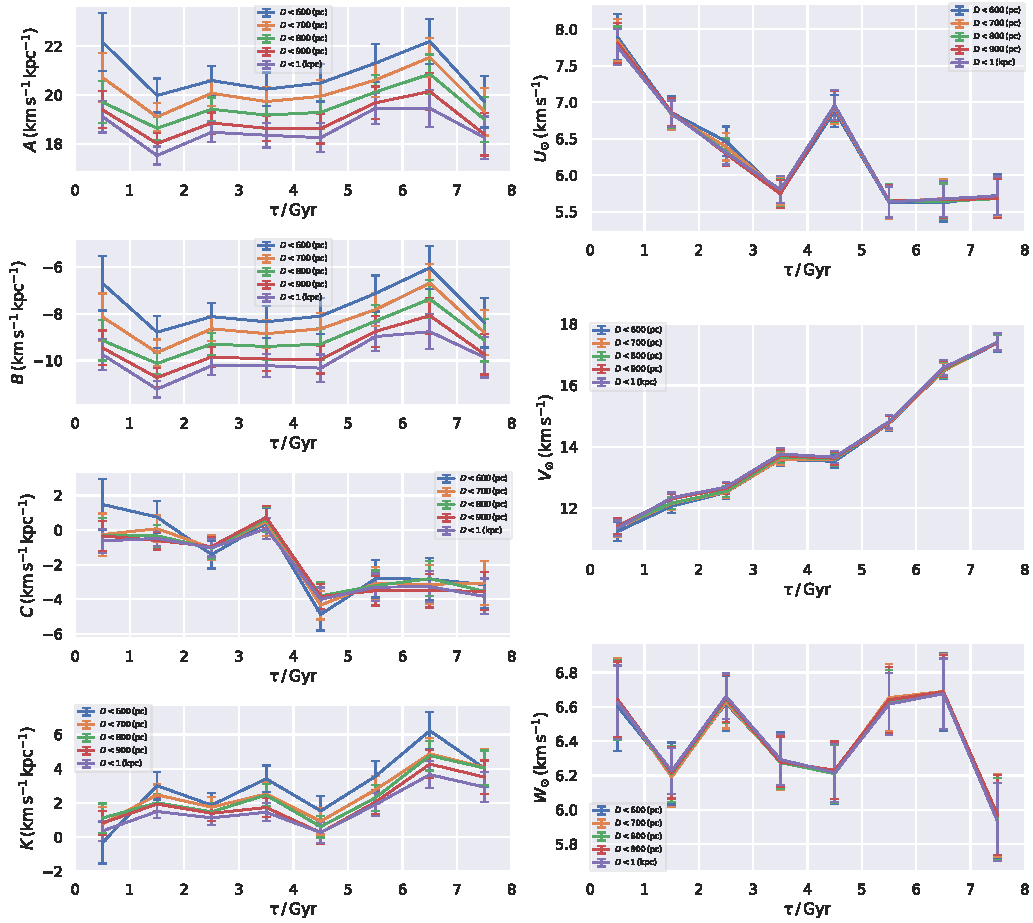
\includegraphics[width=16cm]{fig/Observation_woAD.pdf}
	\caption{asymmetric driftを考慮せずに解析したときのオールト定数と太陽運動の値。}
	\label{fig:woAD}
\end{figure}




\section{asymmetric driftを考慮する場合の解析 \label{asymmetric driftを考慮する場合の解析}}
次に、asymmetric driftを考慮する場合の解析の方法と結果について記述する。ここでは仮定するスケール長の値を変えて全9パターンで解析している。

\subsection{解析方法}
フィッティングパラメータは同様に$A、\,B、\,C、\,K、\,U_{\odot}、\,V_{\odot}、\,W_{\odot}、\,\sigma_{\mu_l}、\,\sigma_{\mu_b}、\,\sigma_{v_{\mathrm{los}}}$の10個である。本解析では、$R_{\odot}$と銀河中心に対する太陽系の回転角速度$\Omega_{g,\odot}=V_{\phi,\odot}/R_{\odot}$について正規分布を仮定して制限する。制限する値には、$R_{\odot}=8.2\pm0.1\,\si{kpc}、\Omega_{g,\odot}=30.24\pm0.12\,\si{km.s^{-1}.kpc}$ (\cite{BH2016})を使用する。このとき$\mathcal{L}$は式(\ref{Likelihood_Mock_AD})を発展させて
\begin{align}
\begin{aligned}
	\ln \mathcal{L} =& -\frac{1}{2}\sum_i \left(\frac{\left[\mu_{l,i} - \mu_l^{\mathrm{AD}}(l_i,b_i,\varpi_i)\right]^2}{\sigma_{\mu_l}^2 + (s_{\mu_{l,i}})^2}  + {\rm ln}\left[\sigma_{\mu_l}^2 + (s_{\mu_{l,i}})^2\right] \right. \\
	&+ \frac{\left[\mu_{b,i} - \mu_b^{\mathrm{AD}}(l_i,b_i,\varpi_i)\right]^2}{\sigma_{\mu_b}^2 + (s_{\mu_{b,i}})^2}  + {\rm ln}\left[\sigma_{\mu_b}^2 + (s_{\mu_{b,i}})^2\right] \\
	&+ \frac{\left[v_{\mathrm{los},i} - v^{\mathrm{AD}}_{\mathrm{los}}(l_i,b_i,\varpi_i)\right]^2}{\sigma_{v_{\mathrm{los}}}^2 + (s_{v_{\mathrm{los},i}})^2} + {\rm ln}\left[\sigma_{v_{\mathrm{los}}}^2 + (s_{v_{\mathrm{los},i}})^2\right]\\
	&+ \frac{\left(R_{\odot} - R_{\odot,\mathrm{prior}}\right)^2}{\sigma_{R_{\odot,\mathrm{prior}}}} + \ln{\sigma_{R_{\odot,\mathrm{prior}}}}\\
	&+ \frac{\left(\Omega_{g,\odot} - \Omega_{g,\odot,\mathrm{prior}}\right)^2}{\sigma_{\Omega_{g,\odot,\mathrm{prior}}}} + \ln{\sigma_{\Omega_{g,\odot,\mathrm{prior}}}}\\
	&+ \left. \frac{\left(\mu_{b,\mathrm{Sgr\,A}^*} - \mu_{b,\mathrm{Sgr\,A}^*,\mathrm{prior}}\right)^2}{\sigma_{\mu_{b,\mathrm{Sgr\,A}^*,\mathrm{prior}}}} + \ln{\sigma_{\mu_{b,\mathrm{Sgr\,A}^*,\mathrm{prior}}}}\right)
\end{aligned} \label{AD10}
\end{align}
と書ける。ここで、$R_{\odot}、\Omega_{g,\odot}$の添字のpriorは仮定している値の平均値、$\sigma_{\mathrm{prior}}$は仮定している値の標準偏差を示す。すなわち、$R_{\odot}$の場合には$R_{\odot,\mathrm{prior}} = 8.2\,\si{kpc}、\,\sigma_{R_{\odot,\mathrm{prior}}}=0.1\,\si{kpc}$である。モデルの式$\mu_l^{\mathrm{AD}}、\mu_b^{\mathrm{AD}}、v^{\mathrm{AD}}_{\mathrm{los}}$は式(\ref{ObsEqAD})を使用している。asymmetric drift速度には式(\ref{AD5})を使用する。式(\ref{AD5})で使用する速度分散$\sigma_R$の計算方法は\ref{asymmetric driftを考慮する場合}と同様であり、また$V_{\phi} = R_{\odot}(A-B)$として計算している。式(\ref{AD10})の最後の行についてはasymmetric driftを考慮しない場合の解析と同様に\cite{RB14}の結果を使用して太陽運動の鉛直方向成分に制限を加えている。

%%%%%%%%%%%%%%%%%%%%%%%%%%%%%%%%

asymmetric driftを考慮する場合の観測方程式(\ref{ObsEqAD})を用いる。ここで、式(\ref{AD5})を
\begin{align}
\begin{aligned}
    v_{\mathrm{a}} &\simeq \frac{\sigma_R^2}{2V_{\phi}} \left[\frac{\sigma_{\phi}^2}{\sigma_R^2} - 1 + R_{\odot}\left(\frac{1}{h_R} + \frac{2}{h_{\sigma}}\right)\right] \\
    &= \frac{\sigma_R^2}{2V_{\phi}} \left[\frac{\sigma_{\phi}^2}{\sigma_R^2} - 1 + \frac{R_{\odot}}{h_R}\left(1 + \frac{2}{h_{\sigma}/h_R}\right)\right]
\end{aligned} \label{AD7}
\end{align}
と変形すると、スケール長のパラメータは$h_R、h_{\sigma}/h_R$の2つとなる。

asymmetric drift速度に式(\ref{AD7})を適用する場合、$\sigma_R、\sigma_{\phi}、V_{\phi}$は観測データから決められることからスケール長は仮定する必要がある。そこで、asymmetric driftを考慮した解析では動径方向の密度と速度分散のスケール長$h_R,h_{\sigma}/h_R$の2パラメータの値で9種類の解析を行っている(表\ref{scalelength})。

\begin{table}
\begin{center}
%\scalebox{0.5}
%\scriptsize
%\footnotesize
%\small
% \begin{tabular}{c|l|c|c|c} \hline
%  \rowcolor{LightCyan}
%  解析名 & Reference & $h_R\ \mathrm{(kpc)}$ & $h_{\sigma}\ \mathrm{(kpc)}$ & 図\\
%  \hline
%   1-a & \multirow{3}{*}{\cite{Piffl14}} & 2.68 & 9 & \ref{figObs1a}\\
%   1-b && 2.68 & $(2\pm 0.5)h_R$ & \\
%   1-c && 2.68 & $(2\pm 0.5)h_R$ & \tabularnewline[\doublerulesep]
%  \hline
%   2-a & \multirow{3}{*}{\cite{SB15}} & 3.45 & 7.8 & \ref{figObs2a}\\
%   2-b && 3.45 & $(2\pm 0.5)h_R$ & \ref{figObs2b}\\
%   2-c && 3.45 & $(2\pm 0.5)h_R$ & \ref{figObs2c} \tabularnewline[\doublerulesep]
%  \hline
%   3-a & \multirow{3}{*}{\cite{BP15}} & 3.66 & $2h_R$ & \ref{figObs3a}\\
%   3-b && 3.66 & $(2\pm 0.5)h_R$ & \ref{figObs3b}\\
%   3-c && 3.66 & $(2\pm 0.5)h_R$ & \ref{figObs3c} \tabularnewline[\doublerulesep]
%  \hline
%   4 & \cite{BP15} & $(3.66 \pm 1.0) + 8 - \tau\ (\mathrm{Gyr})$ & $(2\pm 0.5)h_R$ & \ref{figObs4}\\
%  \hline
%   5 & \cite{BH2016} & $(2.6 \pm 1.0) + 8 - \tau\ (\mathrm{Gyr})$ & $(2\pm 0.5)h_R$ & \ref{figObs5}\\
%  \hline
% \end{tabular}
\begin{tabular}{c|l|c|c} \hline
 \rowcolor{LightCyan}
 解析名 & $h_R\ \mathrm{(kpc)}$ & $ h_{\sigma}/h_R$ & 図\\
 \hline
 1a & $2.6 - 0.5 = 2.1$ & $1.5$ & \ref{figObs1a}\\
 1b & $2.6 - 0.5 = 2.1$ & $2$ & \ref{figObs1b}\\
 1c & $2.6 - 0.5 = 2.1$ & $2.5$ & \ref{figObs1c}\\
 \hline
 2a & $2.6$ & $1.5$ & \ref{figObs2a}\\
 2b & $2.6$ & $2$ & \ref{figObs2b}\\
 2c & $2.6$ & $2.5$ & \ref{figObs2c}\\
 \hline
 3a & $2.6 + 0.5 = 3.1$ & $1.5$ & \ref{figObs3a}\\
 3b & $2.6 + 0.5 = 3.1$ & $2$ & \ref{figObs3b}\\
 3c & $2.6 + 0.5 = 3.1$ & $2.5$ & \ref{figObs3c}\\
 \hline
\end{tabular}
\caption{観測データのasymmetric driftを考慮した解析を行った際に仮定したスケール長 (\cite{BH2016})。\cite{BH2016}ではスケール長を$h_R = 2.6\pm0.5\,\si{kpc}$と結論づけていることから、表のように$1\sigma$の範囲で値を3種類に振った。また、天の川銀河や系外銀河のスケール長の研究から、密度のスケール長$h_R$と速度分散のスケール長$h_{\sigma}$には典型的に$h_R \simeq 2h_{\sigma}$という関係があることが知られているため、$h_{\sigma}/h_R = 2\pm0.5$と考えて、$h_R$と同様に$1\sigma$の範囲で値を3種類に振っている。}
\label{scalelength}
\end{center}
\end{table}


\subsection{解析結果}
本章では、全解析おいて、解析に使うサンプルの太陽からの距離を$\SI{400}{pc}、\SI{700}{pc}、\SI{1}{kpc}$と変更して3パターンの解析を行っている。

まず、解析1aの結果図\ref{figObs1a}はこの解析の結果である。解析1aでは$h_R=1.6\,\si{kpc}、h_{\sigma}/h_R=1.5\,\si{kpc}$として解析した。この結果を見ると、オールト定数$A、B$はほぼ同じ形のプロットとなっており、サンプルの太陽からの距離の範囲で多少の違いはあるが、どの場合も同じようなトレンドが見える。ただ、$D<\SI{400}{pc}$の場合は$\tau<\SI{2}{Gyr}$と星の年齢が若いときには$D<\SI{700}{pc}、D<\SI{1}{kpc}$よりも$\SI{1}{km.s^{-1}.kpc^{-1}}$程度大きい値となっている。また、年齢依存性があり、星が古くなるにつれて値が大きくなっている。$C$は星の年齢が上がるにつれて$C$の値がわずかに小さくなっており、その差は最大で$\SI{6}{km.s^{-1}.kpc^{-1}}$である。しかし、3 Gyrと4 Gyrとの間で値が一度大きくなっている。$K$は$D<\SI{400}{pc}$では星の年齢によって値が大きく変化している一方、$D<\SI{700}{pc}、\SI{1}{kpc}$では$D<\SI{400}{pc}$の結果に比べてあまり変化しておらず、特に6 Gyrまでの星では年齢依存性がほぼなく、値は$\SI{0}{km.s^{-1}.kpc^{-1}}$に近い。$U_{\odot}$は年齢が若いサンプルでは値が大きい。4 Gyrまでは強い年齢依存性があり、その差は最大で$\SI{2}{km.s^{-1}}$程度となっている。$V_{\odot}$ではまだ年齢依存性が見られるが、星の年齢が上がるごとに値が下がり、asymmetric driftを使用しない場合(図\ref{fig:woAD})とは別の傾向となっている。また、値の差は最大で$\SI{3}{km.s^{-1}}$程度ある。サンプルの太陽からの距離の範囲でも値が多少変わり、太陽からの距離の最大値が大きいサンプルほど$V_{\odot}$の値は大きくなっている。

図\ref{1a_triangle}は解析1aで$D<\SI{1}{kpc}$として解析したときの三角プロットである。$A、B$に強い相関が見られる。これは、本論文では太陽系の銀河回転方向の運動速度に正規分布に従う制限を加えているため、太陽系の銀河回転方向の運動速度$V_{\phi,\odot}$が$V_{\phi,\odot}=R_{\phi}(A-B)+V_{\odot}$で表されることから$A-B$の値がほぼ一定となるためであると考えられる。$A$と$V_{\odot}$、$B$と$V_{\odot}$の間の弱い相関も見られ、これも先ほど述べたことに起因していると考えられる。また、$C、 K$間と$K、U_{\odot}$間でも非常に弱い相関が見られる。その他のパラメータ間では大きな相関は見られない。

\begin{figure}
   \centering
\begin{tabular}{cc}
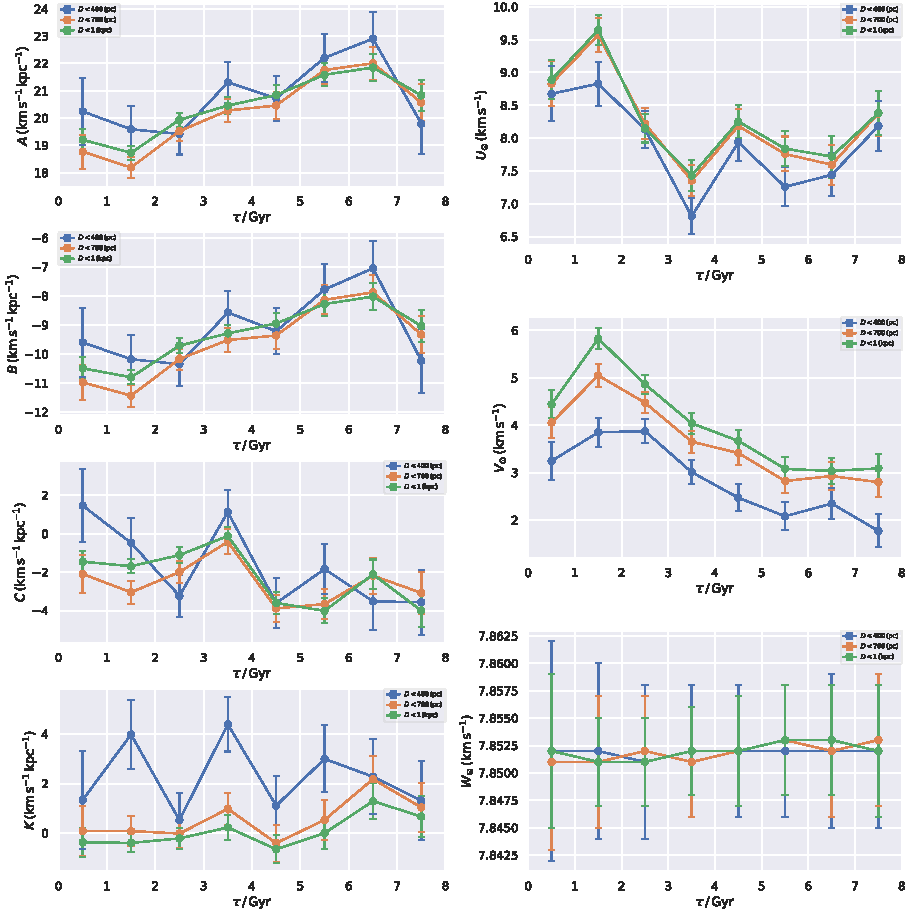
\includegraphics[width=16cm]{fig/1a.pdf}
\end{tabular}
    \caption{(解析1a) $h_R=2.1\,\mathrm{kpc}, h_{\sigma}/h_R=1.5$として解析したときのオールト定数と太陽運動の値。オールト定数$A、B$はほぼ同じ形のプロットとなっており、サンプルの太陽からの距離の範囲で多少の違いはあるが、どの場合も同じようなトレンドが見える。ただ、$D<\SI{400}{pc}$の場合は$\tau<\SI{2}{Gyr}$と星の年齢が若いときには$D<\SI{700}{pc}、D<\SI{1}{kpc}$よりも$\SI{1}{km.s^{-1}.kpc^{-1}}$程度大きい値となっている。また、年齢依存性があり、星が古くなるにつれて値が大きくなっている。$C$は星の年齢が上がるにつれて$C$の値がわずかに小さくなっており、その差は最大で$\SI{6}{km.s^{-1}.kpc^{-1}}$である。しかし、3 Gyrと4 Gyrとの間で値が一度大きくなっている。$K$は$D<\SI{400}{pc}$では星の年齢によって値が大きく変化している一方、$D<\SI{700}{pc}、\SI{1}{kpc}$では$D<\SI{400}{pc}$の結果に比べてあまり変化しておらず、特に6 Gyrまでの星では年齢依存性がほぼなく、値は$\SI{0}{km.s^{-1}.kpc^{-1}}$に近い。$U_{\odot}$は年齢が若いサンプルでは値が大きい。4 Gyrまでは強い年齢依存性があり、その差は最大で$\SI{2}{km.s^{-1}}$程度となっている。$V_{\odot}$ではまだ年齢依存性が見られるが、星の年齢が上がるごとに値が下がり、asymmetric driftを使用しない場合(図\ref{fig:woAD})とは別の傾向となっている。また、値の差は最大で$\SI{3}{km.s^{-1}}$程度ある。サンプルの太陽からの距離の範囲でも値が多少変わり、太陽からの距離の最大値が大きいサンプルほど$V_{\odot}$の値は大きくなっている。}
    \label{figObs1a}
\end{figure}

\begin{figure}
   \centering
\begin{tabular}{cc}
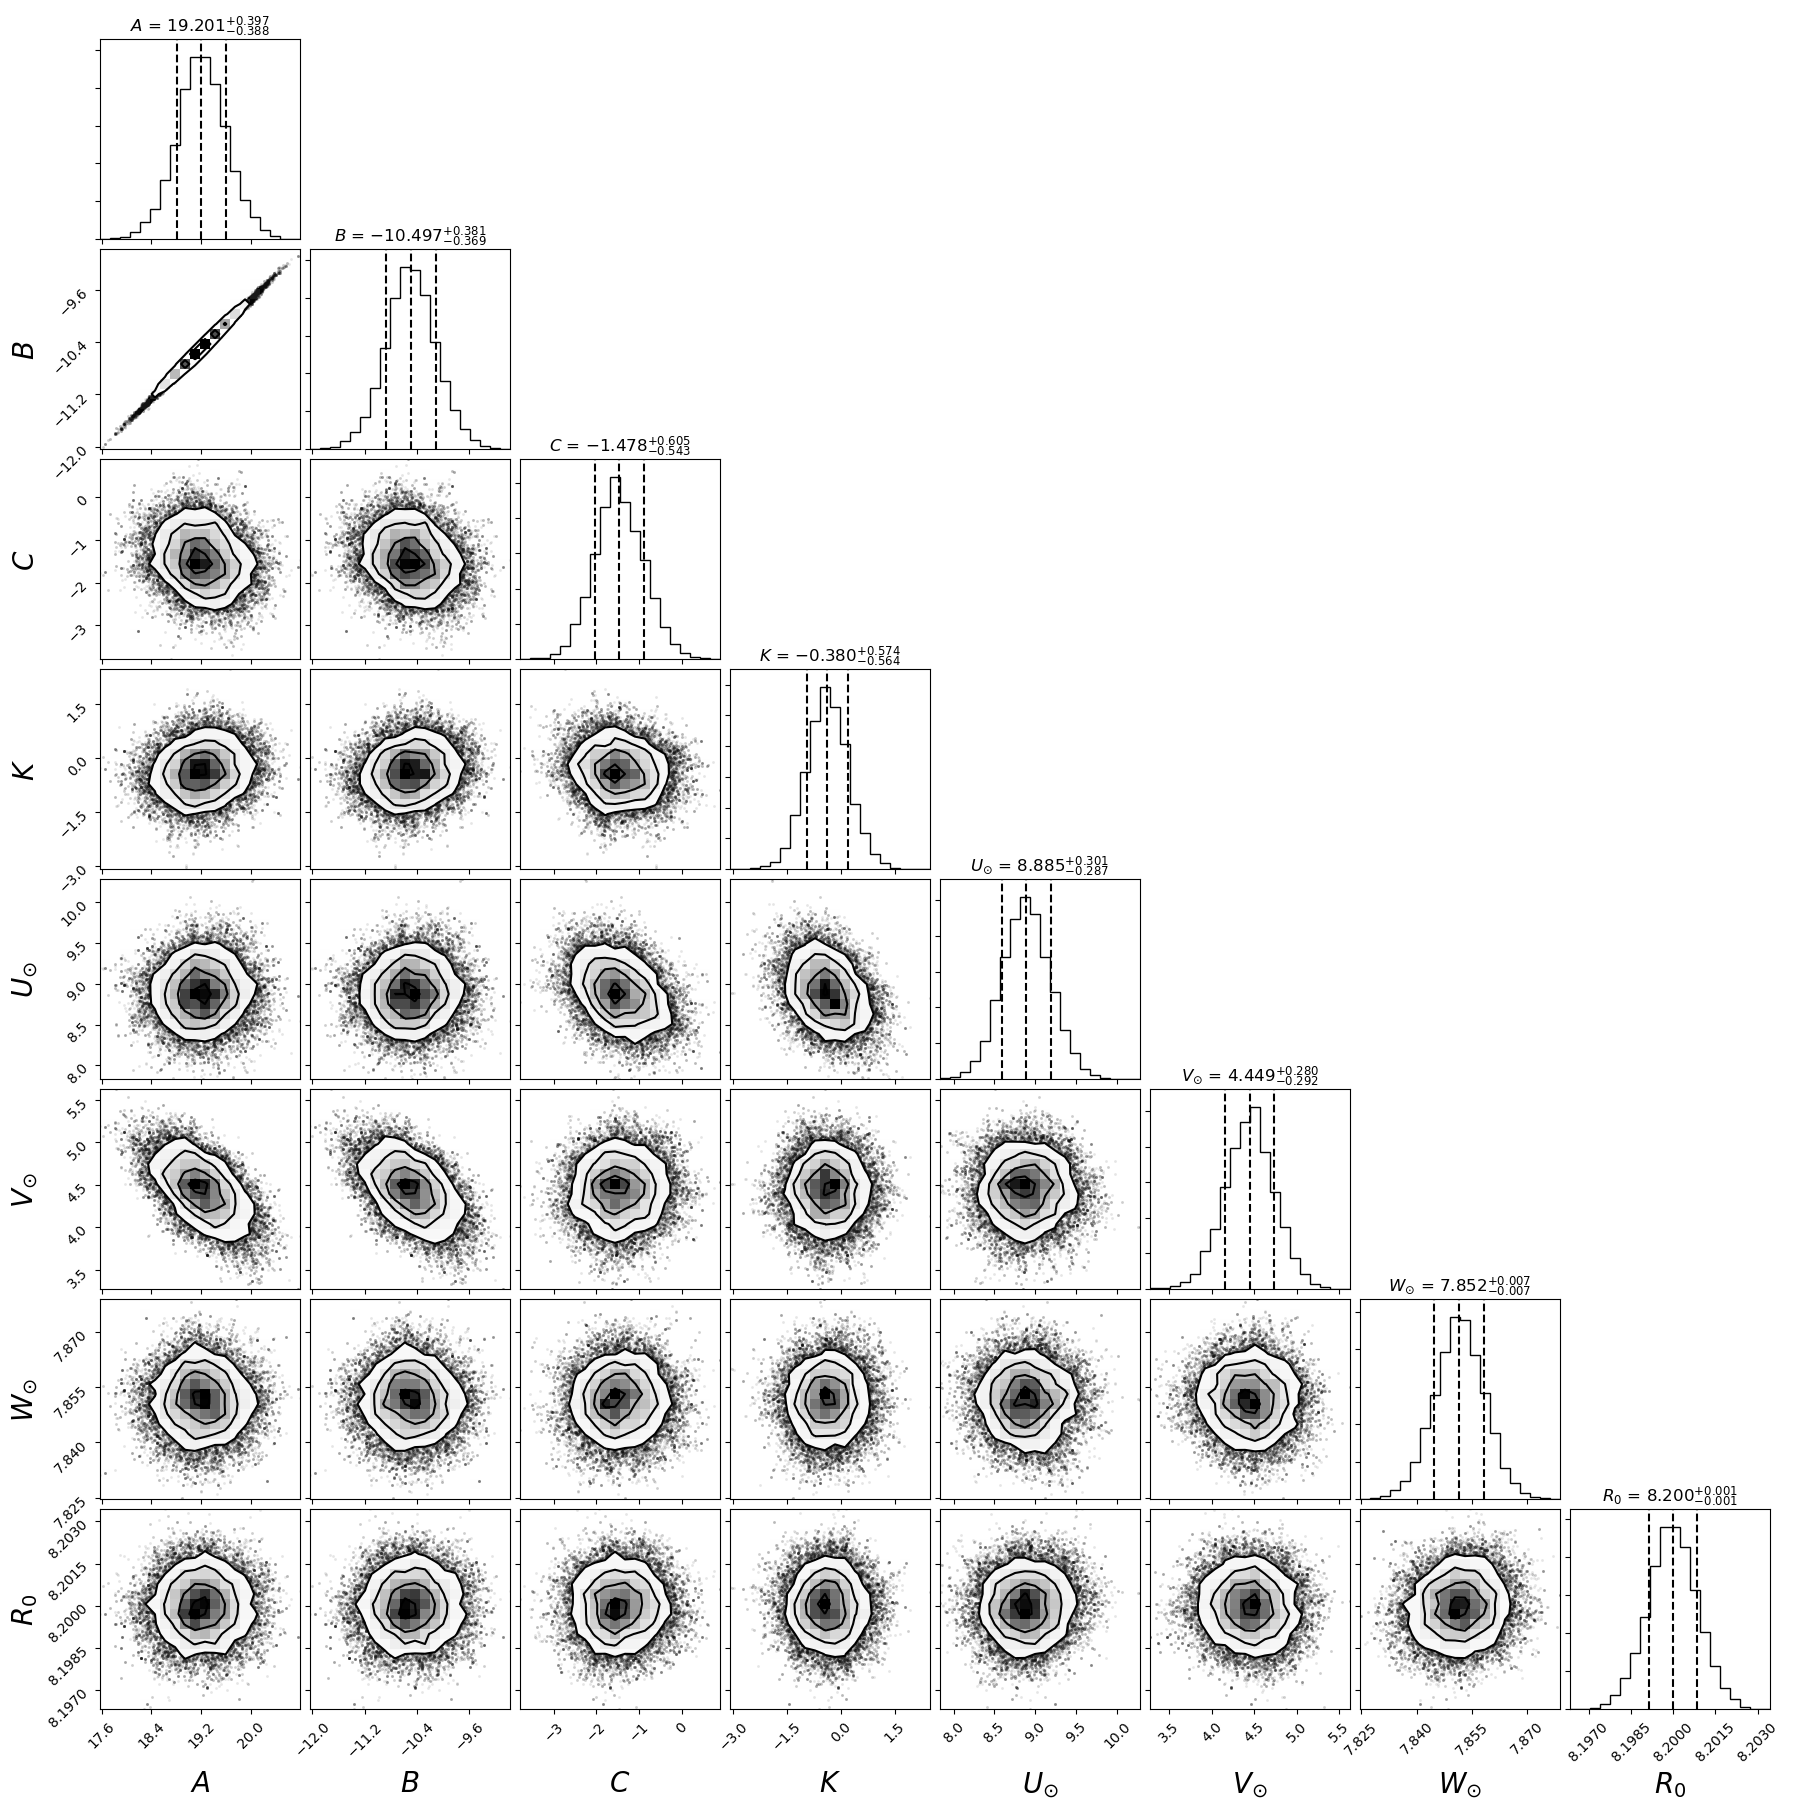
\includegraphics[width=15cm]{fig/1a_triangle.png}
\end{tabular}
    \caption{解析1aの三角プロット。太陽からの距離$\SI{1}{kpc}$以内のサンプルを使用している。各パラメータの頻度分布と各パラメータ間の2次元頻度分布を示している。$A、B$に強い相関が見られる。これは、本論文では太陽系の銀河回転方向の運動速度に正規分布に従う制限を加えているため、太陽系の銀河回転方向の運動速度$V_{\phi,\odot}$が$V_{\phi,\odot}=R_{\phi}(A-B)+V_{\odot}$で表されることから$A-B$の値がほぼ一定となるためであると考えられる。$A$と$V_{\odot}$、$B$と$V_{\odot}$の間の弱い相関も見られ、これも先ほど述べたことに起因していると考えられる。また、$C、 K$間と$K、U_{\odot}$間でも非常に弱い相関が見られる。その他のパラメータ間では大きな相関は見られない。}
    \label{1a_triangle}
\end{figure}

解析1bでは$h_R=1.6\,\si{kpc}、h_{\sigma}/h_R=2\,\si{kpc}$として解析している。図\ref{figObs1b}はこの解析の結果である。オールト定数と$U_{\odot}、W_{\odot}$は解析1aとほぼ同じ結果となっている。$V_{\odot}$は解析1aとは傾向も値も異なり、解析1bでは1aよりも年齢依存性が低くなっている。$D<\SI{400}{pc}、\SI{700}{pc}、\SI{1}{kpc}$のいずれも$\tau=2\,\si{Gyr}$周辺で大きい値となっている。$D$が大きいサンプルの解析結果ほど$V_{\odot}$の値が大きくなっているのは解析1aと同様である。

\begin{figure}
   \centering
\begin{tabular}{cc}
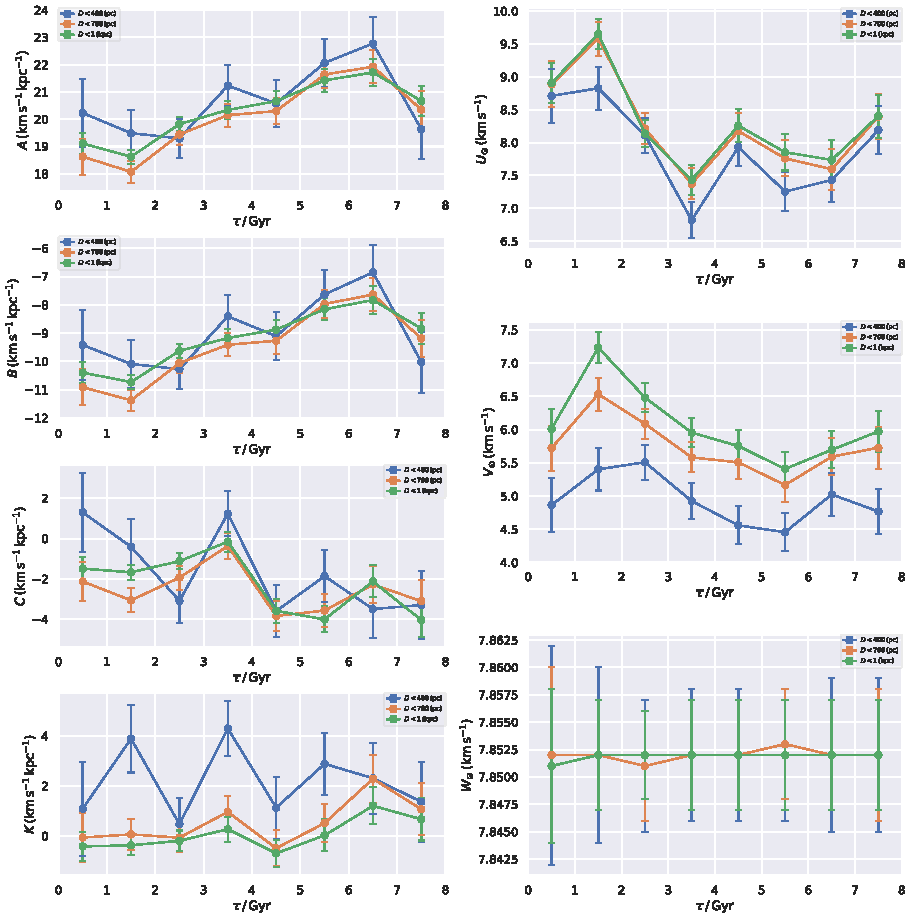
\includegraphics[width=16cm]{fig/1b.pdf}
\end{tabular}
    \caption{(解析1b) $h_R=2.1\,\mathrm{kpc}, h_{\sigma}/h_R=2$として解析したときのオールト定数と太陽運動の値。オールト定数と$U_{\odot}、W_{\odot}$は解析1aとほぼ同じ結果となっている。$V_{\odot}$は解析1aとは傾向も値も異なり、解析1bでは1aよりも年齢依存性が低くなっている。$D<\SI{400}{pc}、\SI{700}{pc}、\SI{1}{kpc}$のいずれも$\tau=2\,\si{Gyr}$周辺で大きい値となっている。$D$が大きいサンプルの解析結果ほど$V_{\odot}$の値が大きくなっているのは解析1aと同様である。}
    \label{figObs1b}
\end{figure}

解析1cでは$h_R=1.6\,\si{kpc}、h_{\sigma}/h_R=2.5\,\si{kpc}$として解析している。図\ref{figObs1c}はこの解析の結果である。解析1bと同様に、オールト定数と$U_{\odot}、W_{\odot}$は解析1aとほぼ同じ結果である一方$V_{\odot}$は解析1a、1bと異なる値となっている。$V_{odot}$の値は$\SI{12.5}{km.s^{-1}}$から$\SI{14.5}{km.s^{-1}}$の間となっており、解析1a、1bよりも大きい値となっている。また、年齢依存性を持っており、解析1aと同様に年齢が上がるほど値が大きい傾向となっている。

\begin{figure}
   \centering
\begin{tabular}{cc}
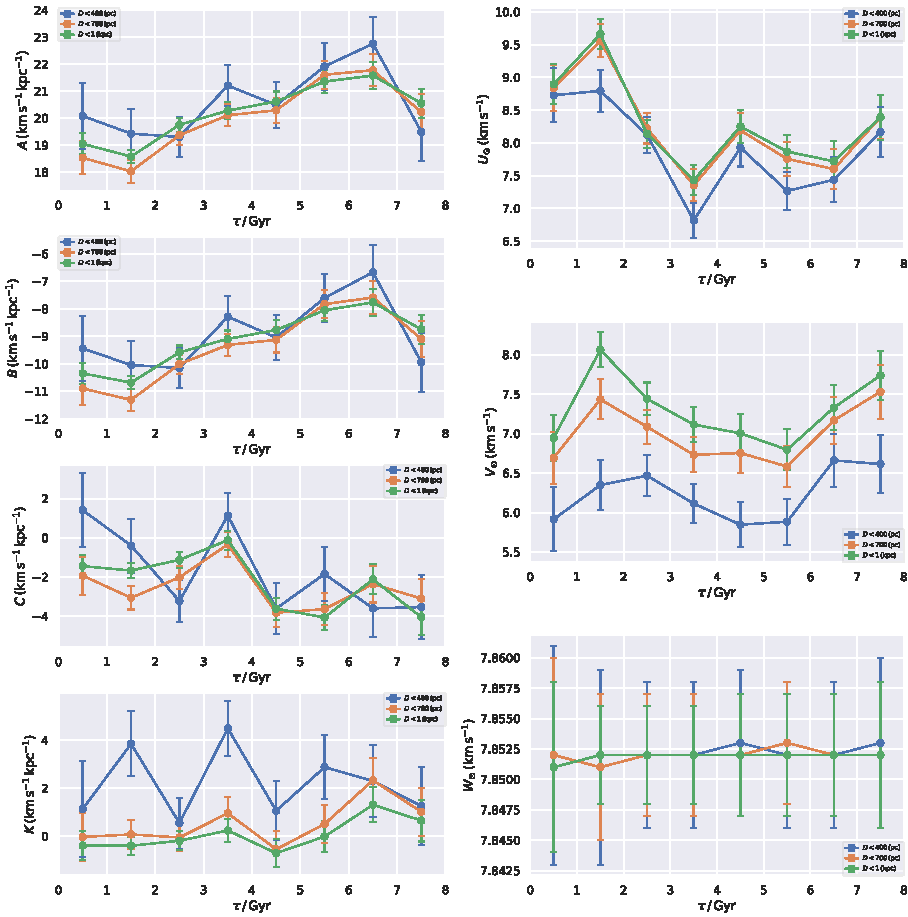
\includegraphics[width=16cm]{fig/1c.pdf}
\end{tabular}
    \caption{(解析1c) $h_R=2.1\,\mathrm{kpc}, h_{\sigma}/h_R=2.5$として解析したときのオールト定数と太陽運動の値。解析1bと同様に、オールト定数と$U_{\odot}、W_{\odot}$は解析1aとほぼ同じ結果である一方$V_{\odot}$は解析1a、1bと異なる値となっている。$V_{odot}$の値は$\SI{12.5}{km.s^{-1}}$から$\SI{14.5}{km.s^{-1}}$の間となっており、解析1a、1bよりも大きい値となっている。また、年齢依存性を持っており、解析1aと同様に年齢が上がるほど値が大きい傾向となっている。}
    \label{figObs1c}
\end{figure}

\begin{figure}
   \centering
\begin{tabular}{cc}
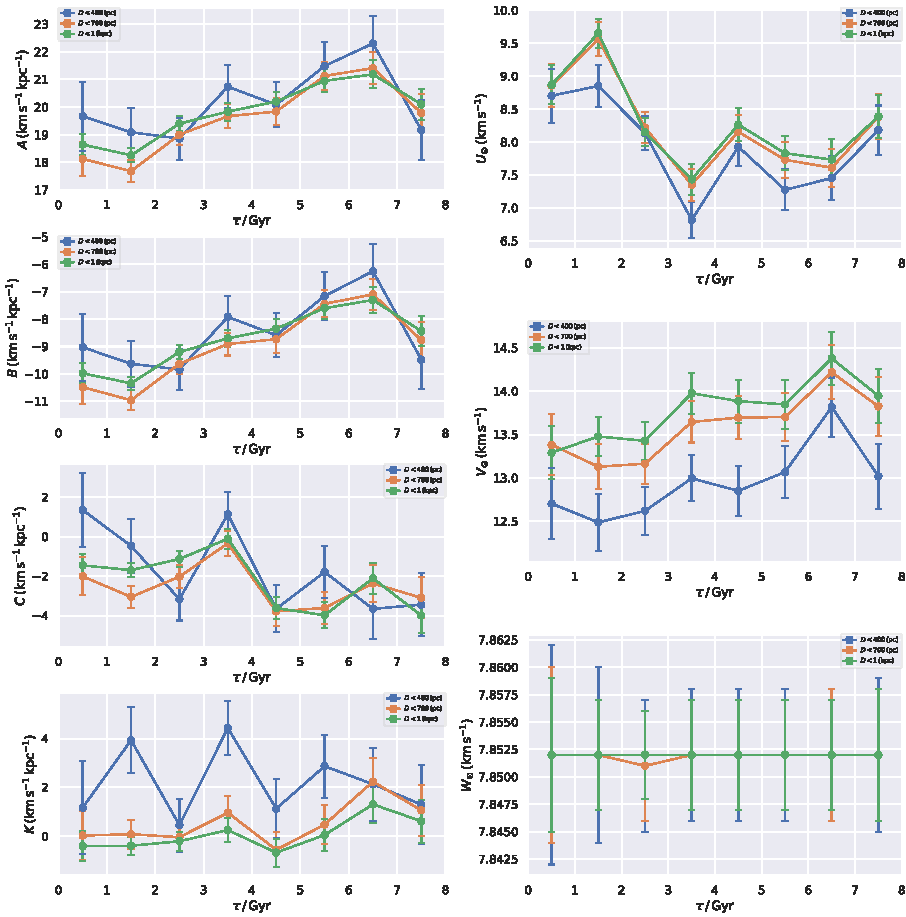
\includegraphics[width=16cm]{fig/2a.pdf}
\end{tabular}
    \caption{(解析2a) $h_R=2.6\,\mathrm{kpc}, h_{\sigma}/h_R=1.5$として解析したときのオールト定数と太陽運動の値。オールト定数と太陽運動$U_{\odot}、W_{\odot}$の値と傾向は解析1a、1b、1cとほぼ同じである。しかし、太陽運動の銀河回転方向成分$V_{\odot}$は値と傾向ともに解析1a、1b、1cとは異なっており、}
    \label{figObs2a}
\end{figure}

\begin{figure}
   \centering
\begin{tabular}{cc}
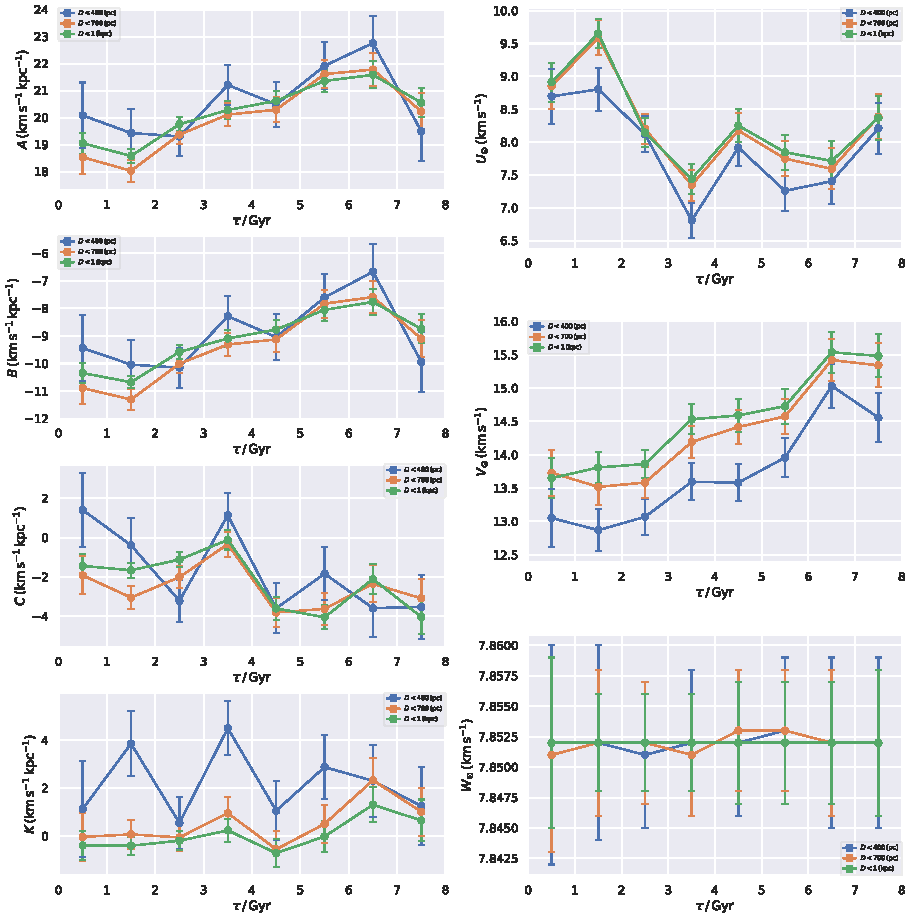
\includegraphics[width=16cm]{fig/2b.pdf}
\end{tabular}
    \caption{(解析2b) $h_R=2.6\,\mathrm{kpc}, h_{\sigma}/h_R=2$として解析したときのオールト定数と太陽運動の値。}
    \label{figObs2b}
\end{figure}

\begin{figure}
   \centering
\begin{tabular}{cc}
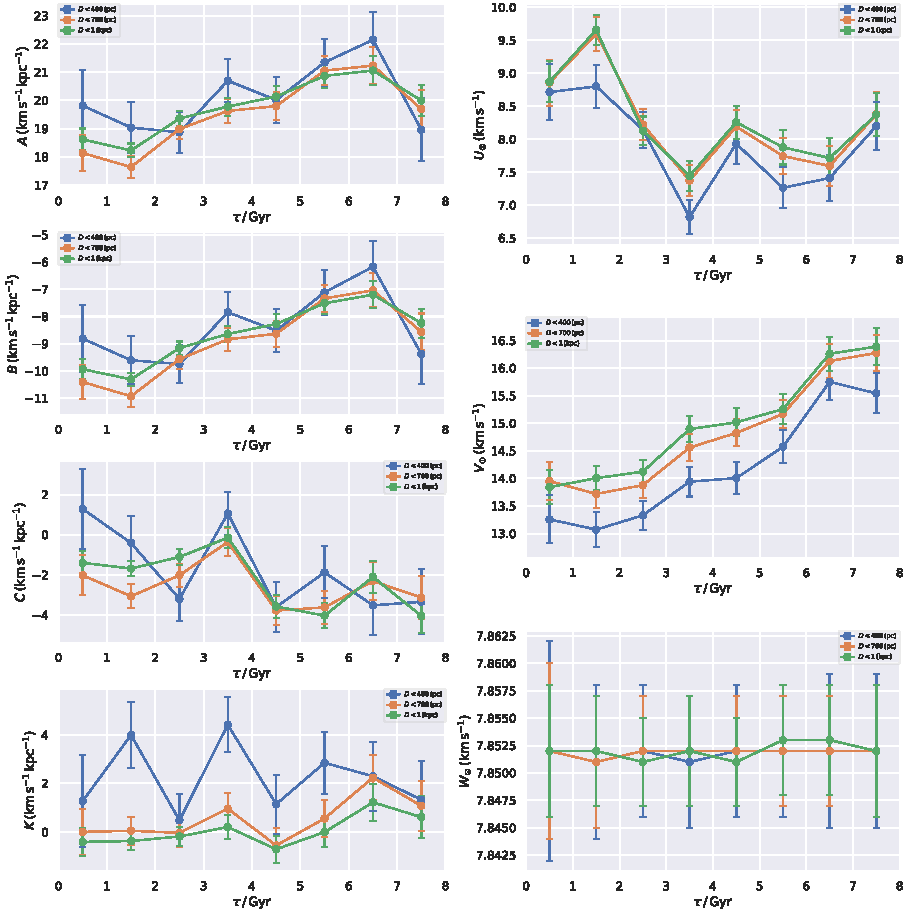
\includegraphics[width=16cm]{fig/2c.pdf}
\end{tabular}
    \caption{(解析2c) $h_R=2.6\,\mathrm{kpc}, h_{\sigma}/h_R=2.5$として解析したときのオールト定数と太陽運動の値。}
    \label{figObs2c}
\end{figure}

\begin{figure}
   \centering
\begin{tabular}{cc}
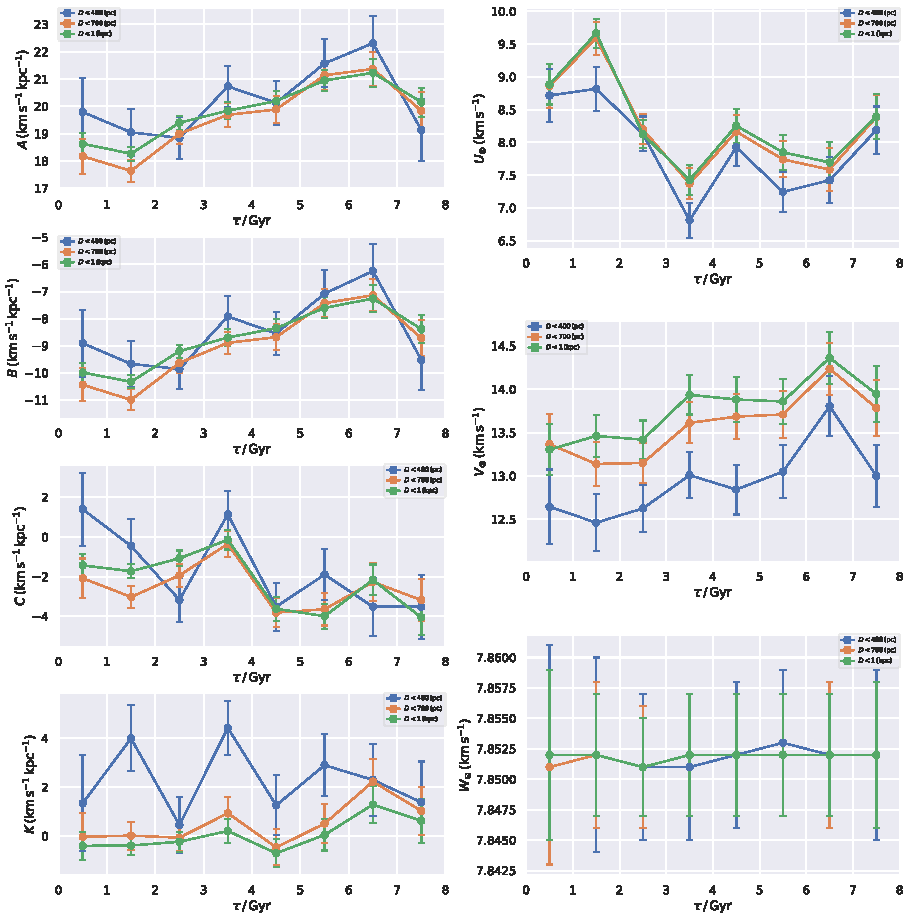
\includegraphics[width=16cm]{fig/3a.pdf}
\end{tabular}
    \caption{(解析3a) $h_R=3.1\,\mathrm{kpc}, h_{\sigma}/h_R=1.5$として解析したときのオールト定数と太陽運動の値。}
    \label{figObs3a}
\end{figure}

\begin{figure}
   \centering
\begin{tabular}{cc}
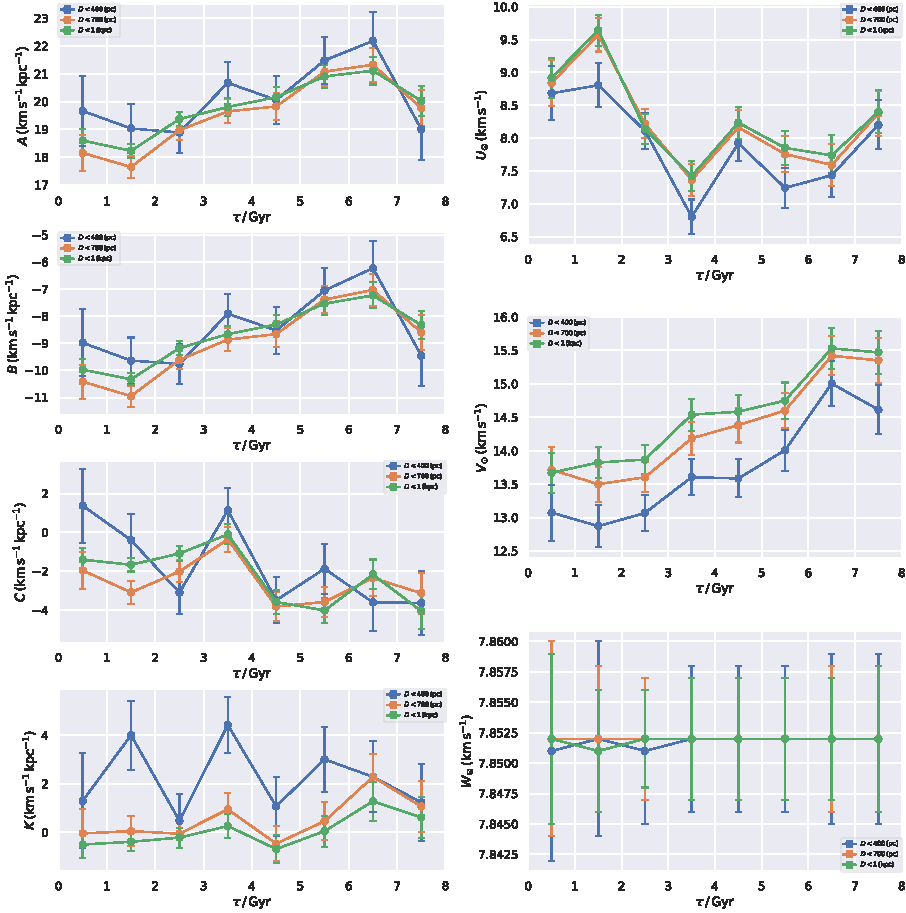
\includegraphics[width=16cm]{fig/3b.pdf}
\end{tabular}
    \caption{(解析3b) $h_R=3.1\,\mathrm{kpc}, h_{\sigma}/h_R=2$として解析したときのオールト定数と太陽運動の値。}
    \label{figObs3b}
\end{figure}

\begin{figure}
   \centering
\begin{tabular}{cc}
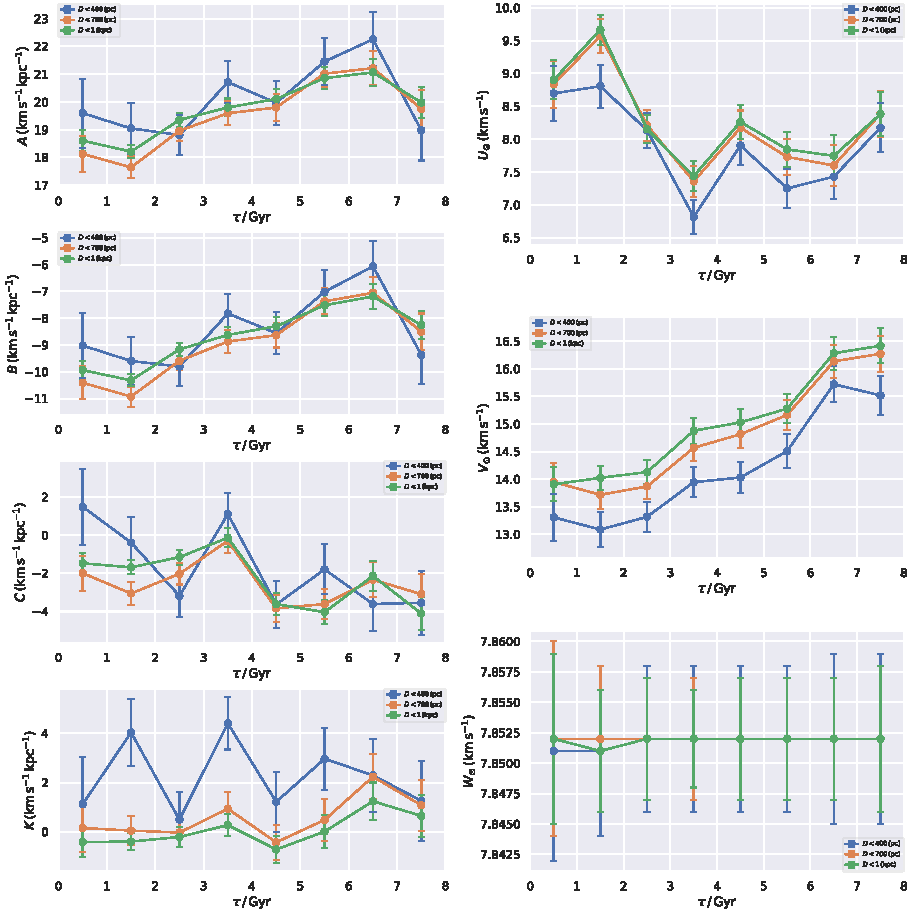
\includegraphics[width=16cm]{fig/3c.pdf}
\end{tabular}
    \caption{(解析3c) $h_R=3.1\,\mathrm{kpc}, h_{\sigma}/h_R=2.5$として解析したときのオールト定数と太陽運動の値。}
    \label{figObs3c}
\end{figure}


% %%%%%%%%%%%%%%%%%%%%%%%%%%%%%%%%%%%%%%%%%%%%%%%%%%%%%%%%%%%%%%%%%%%%%%%%%%%%%%%%%%%%%%%%%%%%%%%%%%%%%%%%
% %%%%%%%%%%%%%%%%%%%%%%%%%%%%%%%%%%%%%%%%%%%%%%%%%%%%%%%%%%%%%%%%%%%%%%%%%%%%%%%%%%%%%%%%%%%%%%%%%%%%%%%%

% 以下は最初に書いていた観測データ解析

% \begin{figure}[htbp]
%   \centering
% \begin{tabular}{cc}
% 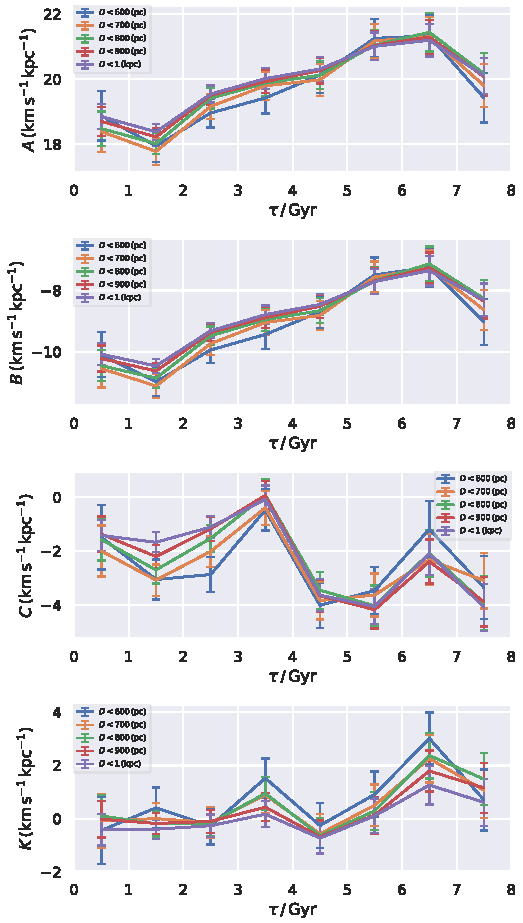
\includegraphics[width=7cm]{fig/ABCK_1a.pdf}
% 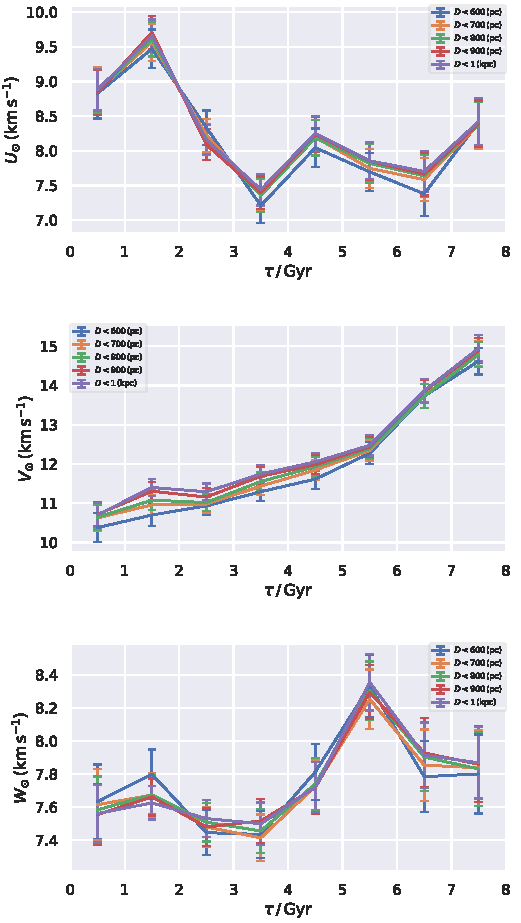
\includegraphics[width=7cm]{fig/UVW_1a.pdf}
% \end{tabular}
%     \caption{(解析1-a) $h_R=2.68\,\mathrm{kpc}, h_{\sigma}=9\,\mathrm{kpc}$として解析したときのオールト定数と太陽運動の値。}
%     \label{figObs1a}
% \end{figure}

% 図\ref{tri1a_0-1}を見ると、$A,B$間で非常に強い相関が見られる。また、若い星の方が古い星よりも$A,B$と$V_{\odot}$との間に負の相関、$C,K$と$U_{\odot}$との間にも弱い負の相関が見られる。

% \begin{figure}[htbp]
% \begin{center}
% 	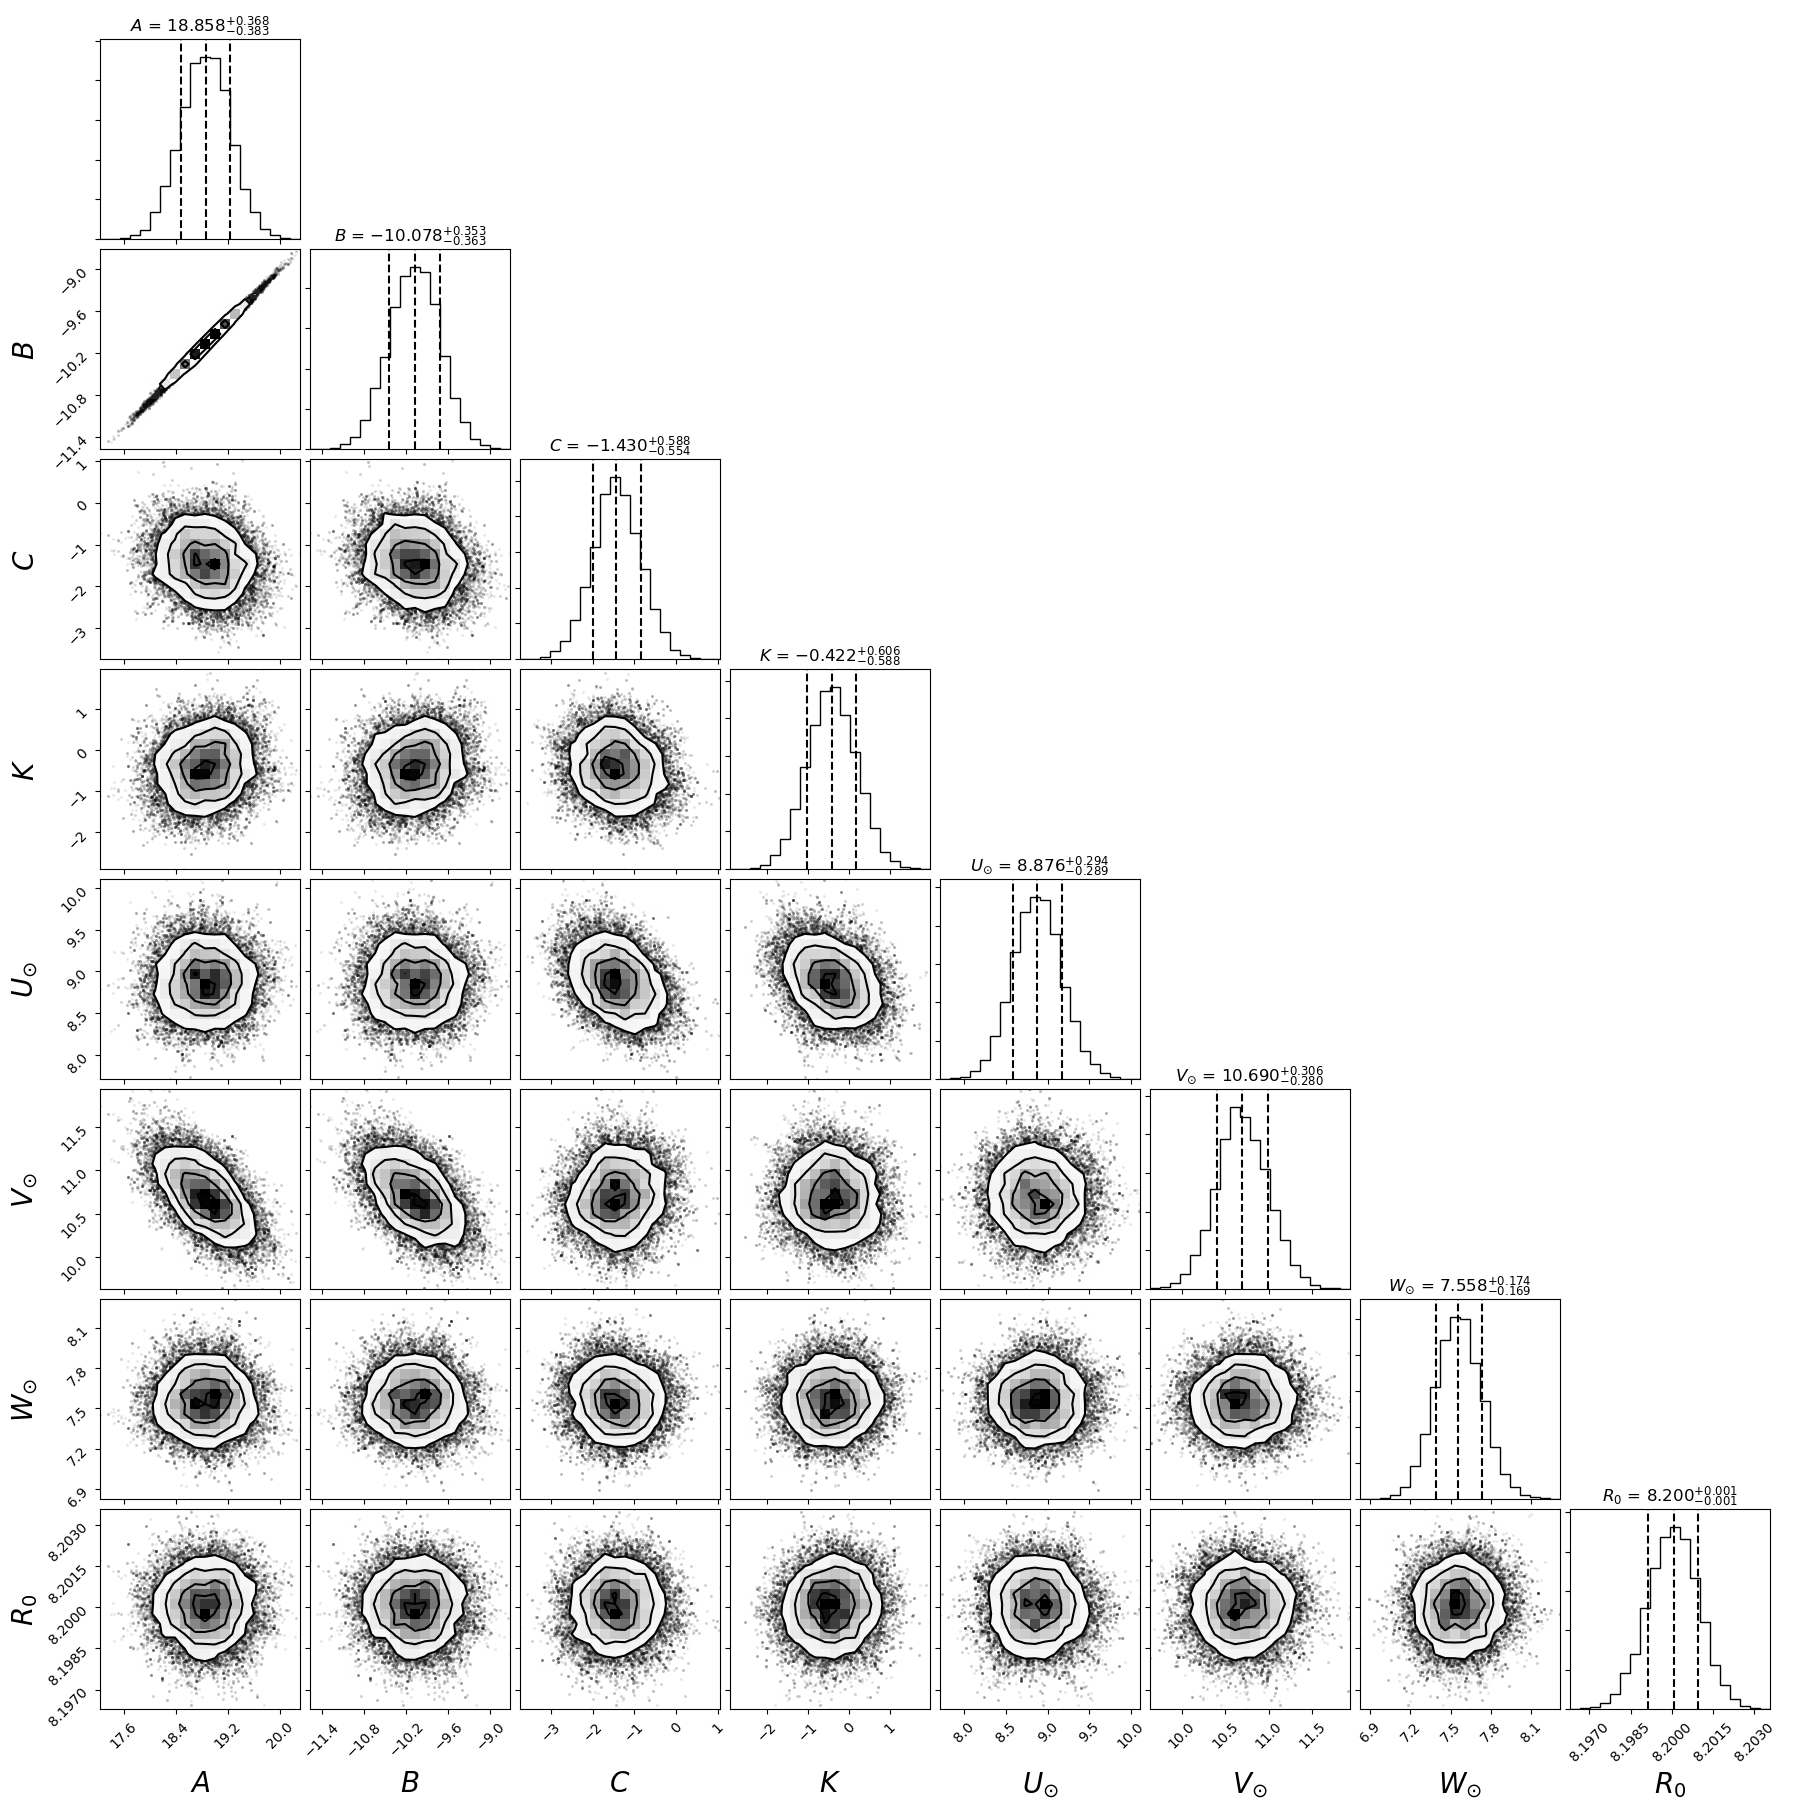
\includegraphics[width=14cm]{fig/1a/trinagle_walker60_Nrun3000_Nburn2000_withscatter_0to1Gyr_1kpc_6076stars_newModel_23.png}
% 	\caption{(解析1-a) 0 - 1 Gyrのサンプルの解析結果のコーナープロット。各パラメータの事後確率分布とそれぞれのパラメータ間の相関を表している。}
% 	\label{tri1a_0-1}
% \end{center}
% \end{figure}

% %%%%%%%%%%%%%%%%%%%%%%%%%%%%%%%%%%%%%%%%%%%%%%%%%%%%%%%%%%%%%%%%%%%%%%%%%%%%%%%%%%%%%%%%%%%%%%%%%%%%%%%%
% %%%%%%%%%%%%%%%%%%%%%%%%%%%%%%%%%%%%%%%%%%%%%%%%%%%%%%%%%%%%%%%%%%%%%%%%%%%%%%%%%%%%%%%%%%%%%%%%%%%%%%%%

% \begin{figure}[htbp]
%   \centering
% \begin{tabular}{cc}
% 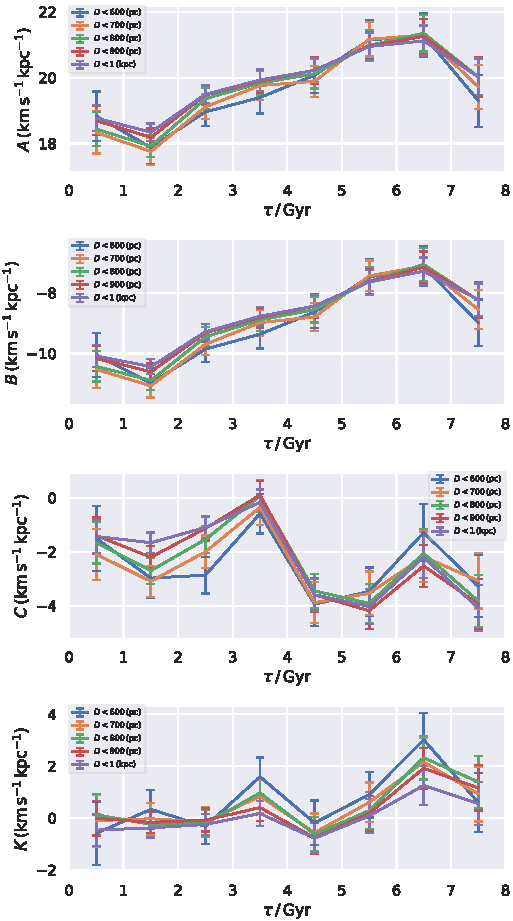
\includegraphics[width=7cm]{fig/ABCK_2a.pdf}
% 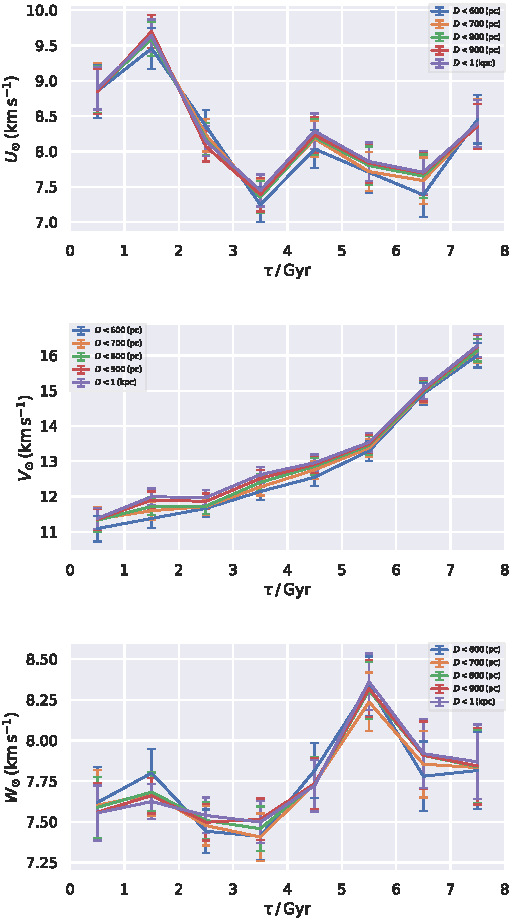
\includegraphics[width=7cm]{fig/UVW_2a.pdf}
% \end{tabular}
%     \caption{(解析2-a) $h_R=3.66\,\mathrm{kpc}, h_{\sigma}=2h_R$として解析したときのオールト定数と太陽運動の値。サンプルの取り方は太陽からの距離の範囲を変えている。}
%     \label{figObs2a}
% \end{figure}

% \begin{figure}[htbp]
%   \centering
% \begin{tabular}{cc}
% 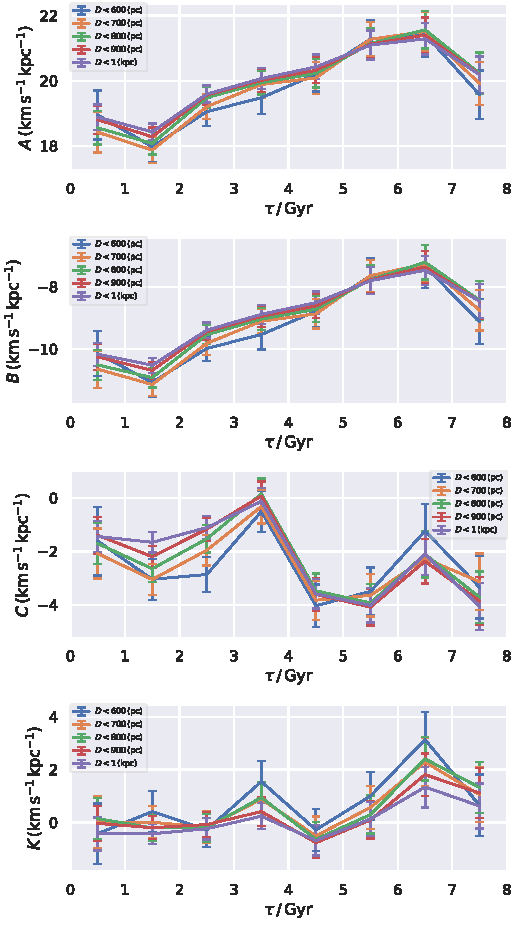
\includegraphics[width=7cm]{fig/ABCK_2b.pdf}
% 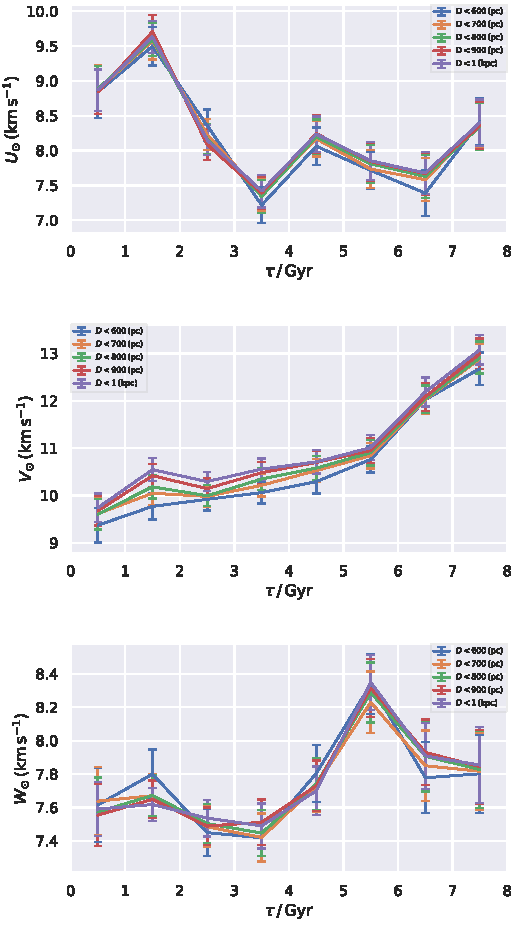
\includegraphics[width=7cm]{fig/UVW_2b.pdf}
% \end{tabular}
%     \caption{(解析2-b) $h_R=3.66\pm 1.0\,\mathrm{kpc},h_{\sigma}=2h_R$として解析したときのオールト定数と太陽運動の値。サンプルの取り方は太陽からの距離の範囲を変えている。}
%     \label{figObs2b}
% \end{figure}

% \begin{figure}[htbp]
%   \centering
% \begin{tabular}{cc}
% 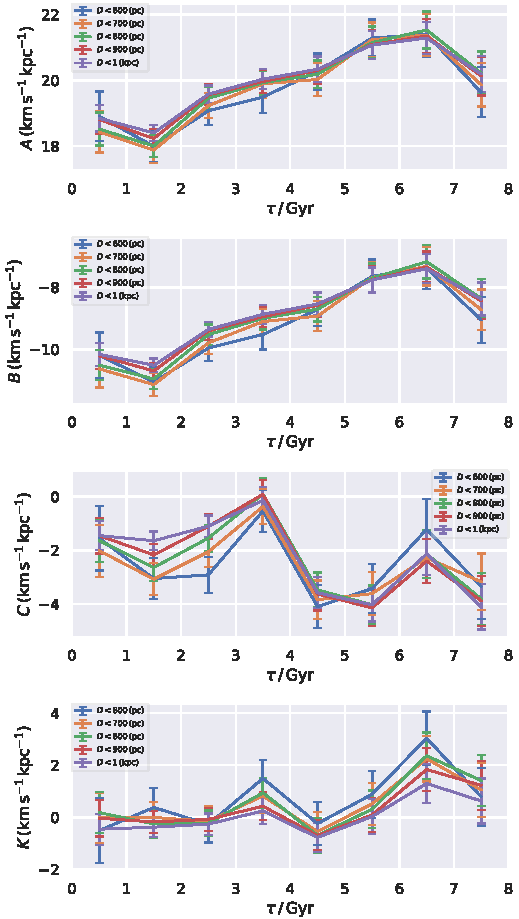
\includegraphics[width=7cm]{fig/ABCK_2c.pdf}
% \includegraphics[width=7cm]{fig/UVW_2c.pdf}
% \end{tabular}
%     \caption{(解析2-c) $h_R=3.66\pm 1.0\,\mathrm{kpc},h_{\sigma}=(2\pm 0.5)h_R$として解析したときのオールト定数と太陽運動の値。サンプルの取り方は太陽からの距離の範囲を変えている。}
%     \label{figObs2c}
% \end{figure}

% %%%%%%%%%%%%%%%%%%%%%%%%%%%%%%%%%%%%%%%%%%%%%%%%%%%%%%%%%%%%%%%%%%%%%%%%%%%%%%%%%%%%%%%%%%%%%%%%%%%%%%%%
% %%%%%%%%%%%%%%%%%%%%%%%%%%%%%%%%%%%%%%%%%%%%%%%%%%%%%%%%%%%%%%%%%%%%%%%%%%%%%%%%%%%%%%%%%%%%%%%%%%%%%%%%

% \begin{figure}[htbp]
%   \centering
% \begin{tabular}{cc}
% \includegraphics[width=7cm]{fig/ABCK_3a.pdf}
% \includegraphics[width=7cm]{fig/UVW_3a.pdf}
% \end{tabular}
%     \caption{(解析3-a) $h_R=3.66\,\mathrm{kpc}, h_{\sigma}=2h_R$として解析したときのオールト定数と太陽運動の値。サンプルの取り方は太陽からの距離の範囲を変えている。}
%     \label{figObs3a}
% \end{figure}

% \begin{figure}[htbp]
%   \centering
% \begin{tabular}{cc}
% \includegraphics[width=7cm]{fig/ABCK_3b.pdf}
% \includegraphics[width=7cm]{fig/UVW_3b.pdf}
% \end{tabular}
%     \caption{(解析3-b) $h_R=3.66\pm 1.0\,\mathrm{kpc},h_{\sigma}=2h_R$として解析したときのオールト定数と太陽運動の値。サンプルの取り方は太陽からの距離の範囲を変えている。}
%     \label{figObs3b}
% \end{figure}

% \begin{figure}[htbp]
%   \centering
% \begin{tabular}{cc}
% \includegraphics[width=7cm]{fig/ABCK_3c.pdf}
% \includegraphics[width=7cm]{fig/UVW_3c.pdf}
% \end{tabular}
%     \caption{(解析3-c) $h_R=3.66\pm 1.0\,\mathrm{kpc},h_{\sigma}=(2\pm 0.5)h_R$として解析したときのオールト定数と太陽運動の値。サンプルの取り方は太陽からの距離の範囲を変えている。}
%     \label{figObs3c}
% \end{figure}


% %%%%%%%%%%%%%%%%%%%%%%%%%%%%%%%%%%%%%%%%%%%%%%%%%%%%%%%%%%%%%%%%%%%%%%%%%%%%%%%%%%%%%%%
% %%%%%%%%%%%%%%%%%%%%%%%%%%%%%%%%%%%%%%%%%%%%%%%%%%%%%%%%%%%%%%%%%%%%%%%%%%%%%%%%%%%%%%%
% %%%%%%%%%%%%%%%%%%%%%%%%%%%%%%%%%%%%%%%%%%%%%%%%%%%%%%%%%%%%%%%%%%%%%%%%%%%%%%%%%%%%%%%

% \begin{figure}[htbp]
%   \centering
% \begin{tabular}{cc}
% \includegraphics[width=7cm]{fig/ABCK_4.pdf}
% \includegraphics[width=7cm]{fig/UVW_4.pdf}
% \end{tabular}
%     \caption{(解析4) $(3.66 \pm 1.0) + 8 - \tau\ (\mathrm{Gyr}), h_{\sigma} = (2\pm 0.5)h_R$として解析したときのオールト定数と太陽運動の値。サンプルの取り方は太陽からの距離の範囲を変えている。}
%     \label{figObs4}
% \end{figure}

% \begin{figure}[htbp]
%   \centering
% \begin{tabular}{cc}
% \includegraphics[width=7cm]{fig/ABCK_5.pdf}
% \includegraphics[width=7cm]{fig/UVW_5.pdf}
% \end{tabular}
%     \caption{(解析5) $(2.6 \pm 1.0) + 8 - \tau\ (\mathrm{Gyr}), h_{\sigma} = (2\pm 0.5)h_R$解析したときのオールト定数と太陽運動の値。サンプルの取り方は太陽からの距離の範囲を変えている。}
%     \label{figObs5}
% \end{figure}

%%%%%%%%%%%%%%%%%%%%%%%%%%%%%%%%%%%%%%%%%%%%%%%%%%%%%%%%%%%%%%%%%%%%%%%%%%%%%%%%%%%%%%%
%%%%%%%%%%%%%%%%%%%%%%%%%%%%%%%%%%%%%%%%%%%%%%%%%%%%%%%%%%%%%%%%%%%%%%%%%%%%%%%%%%%%%%%
%%%%%%%%%%%%%%%%%%%%%%%%%%%%%%%%%%%%%%%%%%%%%%%%%%%%%%%%%%%%%%%%%%%%%%%%%%%%%%%%%%%%%%%

\section{解析結果のまとめ}
図\ref{multi}は太陽から1 kpc以内のサンプルを使用したときのasymmtric driftを考慮しない場合の解析 (no AD)とasymmetric driftを考慮する場合の各解析のプロットである。この結果を見ると、全ての解析パラメータにおいてasymmetric drift考慮しない場合と考慮する場合とで明確に違いが出た。$A、B$はasymmetirc driftを考慮する場合の方が考慮しない場合よりも値が大きくなっている。オールト定数$C、K$と太陽運動$U_{\odot}、W_{\odot}$についてはasymmetric driftを考慮する場合の解析ではほぼ同じ結果となった。それ以外の$A、B、V_{\odot}$はasymmetric driftを考慮する場合の解析の中でも違いが出ており、解析1と解析2、3との間に差がある。ただし、$A、B$はそれらの間でトレンドは変わっていない。$C$はasymmetric driftを考慮する場合としない場合とで傾向が似ており、値も大きな違いはない。$K$はasymmetirc driftを考慮しない場合の方が考慮する場合よりも大きな値となっているが、トレンドは似ている。太陽運動の動径方向成分$U_{\odot}$はasymmetric driftを考慮する場合の方が考慮しない場合よりも値が大きくなっている。太陽運動の銀河回転成分$V_{\odot}$は解析によって最も大きく値に差が出ている。特に、解析1a、1b、1cのスケール長を$h_R=\SI{1.6}{km.s^{-1}}$としている解析では値が$\SI{3}{km.s^{-1}}$から$\SI{8}{km.s^{-1}}$程度と他の場合に比べて小さくなっている。また、asymmetric driftを考慮する場合の解析において、値が小さいパターンほど星の年齢が上がるにつれて値が小さくなる傾向にあり、逆に値が大きいパターンでは逆の傾向がある。

\begin{figure}[htbp]
\begin{center}
	\includegraphics[width=15cm]{fig/multi.pdf}
	\caption{太陽から1 kpc以内のサンプルを使用したときのasymmtric driftを考慮しない場合の解析 (no AD)とasymmetric driftを考慮する場合の各解析のプロット。各線の色と解析方法の対応関係のラベルは図の上部に記載している。解析方法の詳細は表\ref{scalelength}を参照。}
	\label{multi}
\end{center}
\end{figure}